% !TeX spellcheck = it_IT
\newpage
\section{Integrali}
\begin{wrapfigure}[5]{r}{5.5cm}
    \vspace{-25pt}
    \centering
    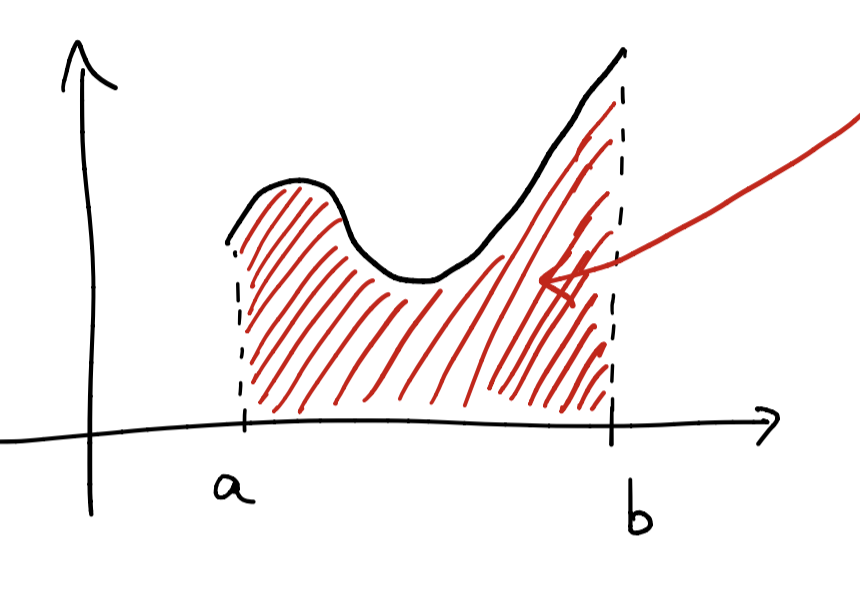
\includegraphics[width=4cm]{images/area-sottografico.png}
\end{wrapfigure}
In questo corso tratteremo gli integrali detti \textbf{di Riemain}.
Sia $f: [a,b] \to \mathbb{R}$, limitata. (ad esempio una funzione continua). L'idea della definizione è che l'integrale (definito) di $f(x)$ in $[a,b]$ rappresenta l'area del sotto grafo di $f$  (questo è vero se $f \geq 0$ su $[a,b]$).

\begin{definition}[Suddivisione di un intervallo]
Una \textbf{suddivisione} di [a,b] è un insieme di $A = \{x_0, x_1, ..., x_n\}$ con $a = x_0 < x_1 < x:2 < ... < x_n = b$.
\end{definition}
\begin{observation}
Le lunghezze degli intervalli $[x_{i-1}, x_u]$ non sono necessariamente uguali.\\
Inoltre $\sum\limits_{i=1}^n(x_i - x_{i-1}) = b - a = $ lunghezza di $[a,b]$.
\end{observation}

\begin{definition}[Somma inferiore]
Dato una suddivisione di un intervallo A, si dice somma inferiore di $f$ relativa alla suddivisione di A 
\vspace{-5pt}
\[S'(f,A) = \sum^n\limits_{i=1} \big( \inf(f(x))_{x \in [x_{i-1}, x_i]} \big) \cdot (x_i - x_{i - 1})\]
\end{definition}
E la somma delle aree dei rettangoli rossi. Approssima l'area del sotto grafico di $f(x)$ per difetto.
\begin{definition}[Somma superiore]
Dato una suddivisione di un intervallo A, si dice somma superiore di $f$ relativa alla suddivisione di A 
\vspace{-5pt}
\[S'(f,A) = \sum^n\limits_{i=1} \big( \sup(f(x))_{x \in [x_{i-1}, x_i]} \big) \cdot (x_{i-1} - x_i)\]
\end{definition}
Somma delle aree dei rettangoli rossi. Questa volta è un'approssimazione per eccesso dell'area del sotto grafico.
\begin{observation}
Non server che $f$ sia continua per dare tutte queste definizione, ma soltanto che sia limitata.
\end{observation}
\begin{definition}[Somme indipendente dalle suddivisioni]
Le somme inferiori e superiori indipendenti dalle suddivisioni si definiscono come:
\begin{itemize}
    \item $S'(f) = sup\{S'(f,A) \:\: |$ A suddivisione di $[a,b]\}$ si dice somma inferiore di $f$.
    \item $S''(f) = inf\{S'(f,A) \:\: |$ A suddivisione di $[a,b]\}$ si dice somma superiore di $f$.
\end{itemize}
\end{definition}
Aggiungendo punti le somme inferiori crescono (e le somme superiori calano).

\begin{figure}[h!]
    \begin{subfigure}{.3\textwidth}
        \centering
        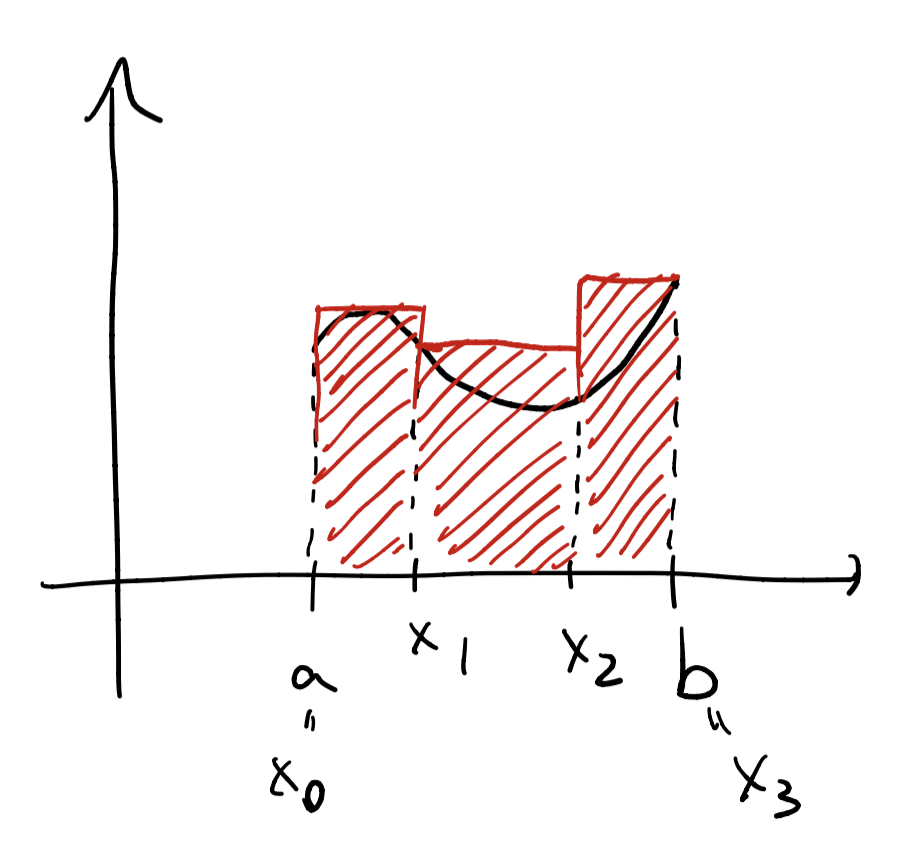
\includegraphics[width=4cm]{somma-superiore.png}
        \caption{Somma superiore}
    \end{subfigure}
    \begin{subfigure}{.3\textwidth}
        \centering
        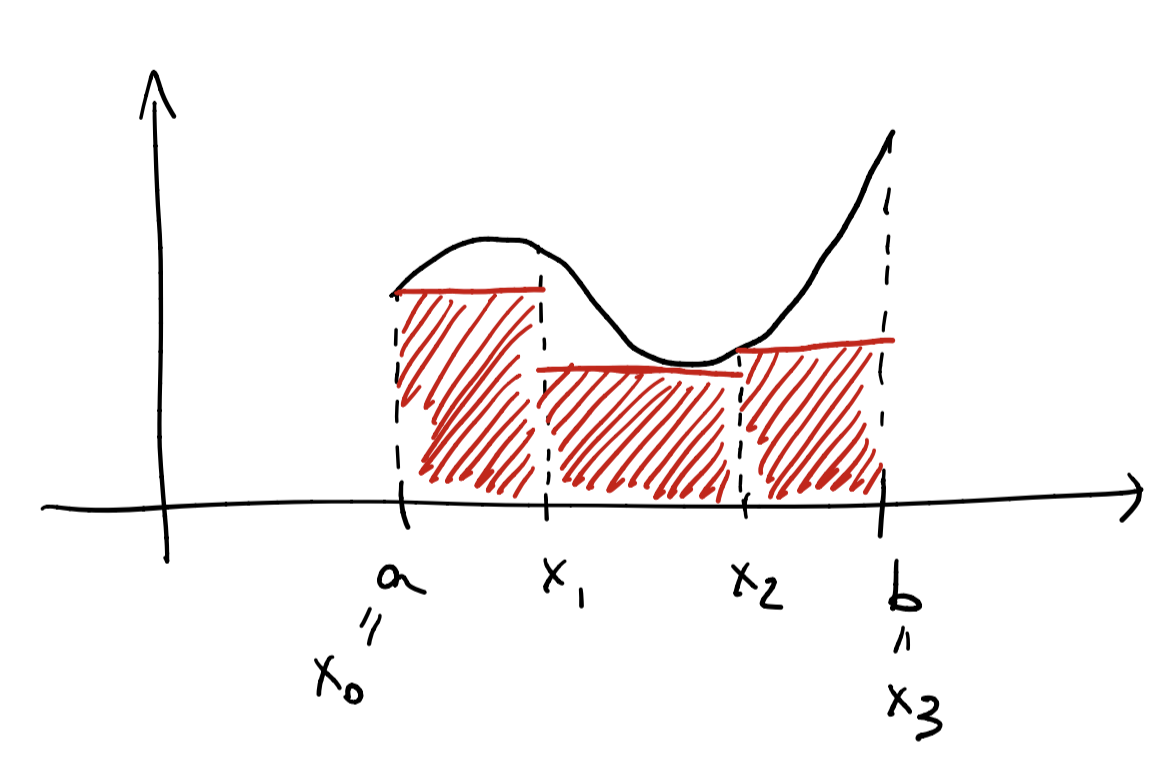
\includegraphics[width=4.5cm]{somma-inferiore.png}
        \caption{Somma inferiore}
    \end{subfigure}
    \begin{subfigure}{.3\textwidth}
        \centering
        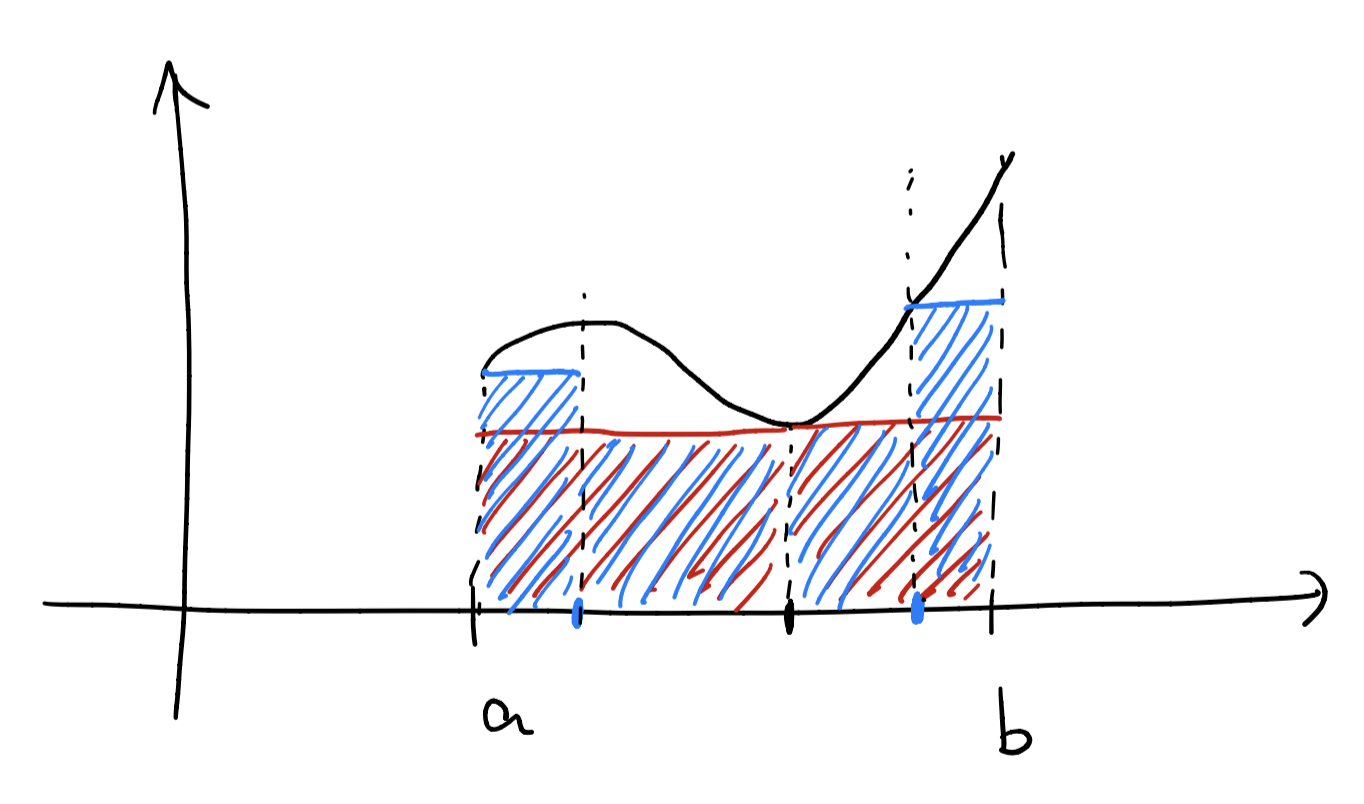
\includegraphics[width=4.5cm]{somma-indipendente.png}
        \caption{Somma indipendente}
    \end{subfigure}
    \caption{Somme delle sezioni}
\end{figure}

\begin{definition}[Integrabile secondo Rieman]
Se $S'(f) = S''(f)$ si dice che $f$ è \textbf{integrabile secondo Rieman} su $[a,b]$ e il valore comune si dice integrale di $f$ su $[a,b]$ e si indica come:
\[\int_{a}^b f(x)\:dx \: \: = S'(f) = S''(f)\]
\end{definition}
\newpage
\begin{observation}
Questa definizione ha senso anche quando $f$ può prendere anche valori negativi.
\end{observation}
\begin{wrapfigure}[4]{r}{6cm}
    \vspace{-15pt}
    \centering
    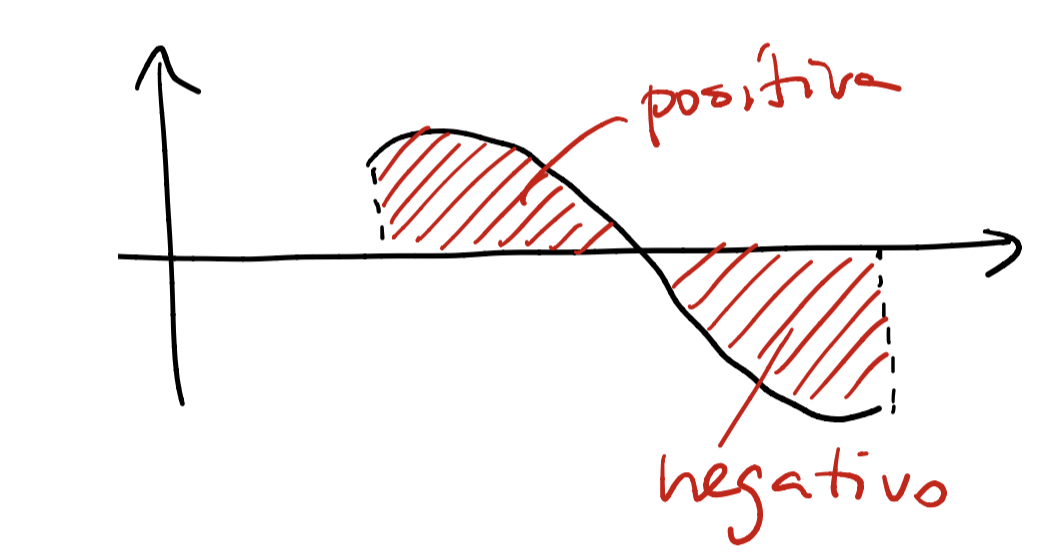
\includegraphics[width=5cm]{images/area-positiva-negativa.png}
\end{wrapfigure}
Se $f \leq 0 \Longrightarrow \int_a^b f(x)\:dx \leq 0$ ed è l'opposto dell'area in figura.
In generale $\int_a^b f(x)\:dx$ è la somma algebrica delle aree in figura (si sommano le aree dove l'integrale è positivo e si sottraggono quelle dove è negativo). \\

\begin{theorem}
Se $f: [a,b] \to \mathbb{R}$ è continua, allora è integrabile.
\end{theorem}

\begin{observation}
Ci sono anche funzioni non continue che sono integrabili, ad esempio una funzione con un punto in cui c'è un salto.
\end{observation}

\begin{definition}
Una $f: [a,b] \to \mathbb{R}$ è generalmente continua se è limitata e ha eventualmente un numero finito di punti di discontinuità.
\end{definition}

\begin{example}
Funzione non generalmente continua. $f(x) = \begin{cases}\frac{1}{x} & x\neq 0 \\ 0 & x=0\end{cases}$ con $f: [-1,1] \to \mathbb{R}$
\\C'è un solo punto di discontinuità, ma $f$ non è limitata $\Longrightarrow$ non è generalmente continua.
\end{example}

\begin{theorem}
Se $f:[a,b] \to \mathbb{R}$ è generalmente continua, allora f è integrabile.
\end{theorem}

\begin{example}
$f(x) = \begin{cases}\sin\frac{1}{x} & x\neq 0 \\ 0 & x=0\end{cases}$ con $f: [0,1] \to \mathbb{R}$.\\
$f(x)$ non è continua ma è generalmente continua $\Longrightarrow$ integrabile
\end{example}

\begin{example}
Esempio di una funzione non integrabile. (Esempio con la funzione di Dirichlet).
\end{example}
\begin{wrapfigure}[7]{r}{5cm}
    \vspace{-25pt}
    \centering
    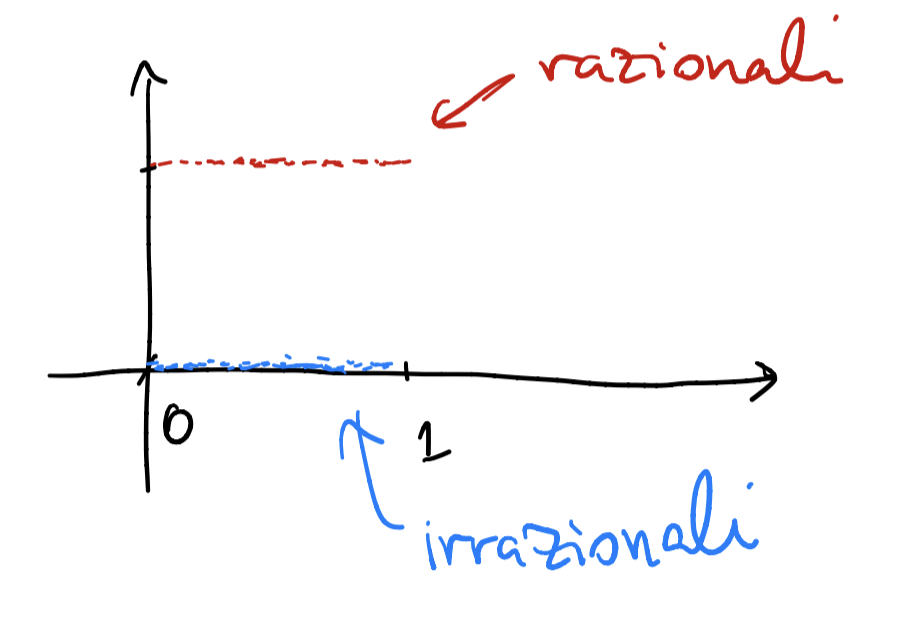
\includegraphics[width=5cm]{images/funzione-dirichlet.png}
\end{wrapfigure}
$f(x) = \begin{cases}1 & x\in\mathbb{Q} \\ 0 & x \notin \mathbb{Q} \end{cases}$ con $f: [0,1] \to \mathbb{R}$.\\
Per qualsiasi intervallo $[x_{i-1}, x_i] \subseteq [0,1]$ si ha che:\\\\
$sup(f(x))_{x \in [x_{i-1}, x_i]} = 1$ e $inf(f(x))_{x \in [x_{i-1}, x_i]} = 0$. \\
Segue che $S'(f,A) = 0 \:\: \forall A$ suddivisione di $[0,1] \Longrightarrow S'(f) = 0$ e $S''(f,A) = 1 \:\: \forall A $ suddivisione di $[0,1] \Longrightarrow S''(f) = 1$. Quindi $S'(f) \neq S''(f) \Longrightarrow f$ non è integrabile.\\\\

\begin{wrapfigure}[3]{l}{5cm}
    \vspace{-30pt}
    \centering
    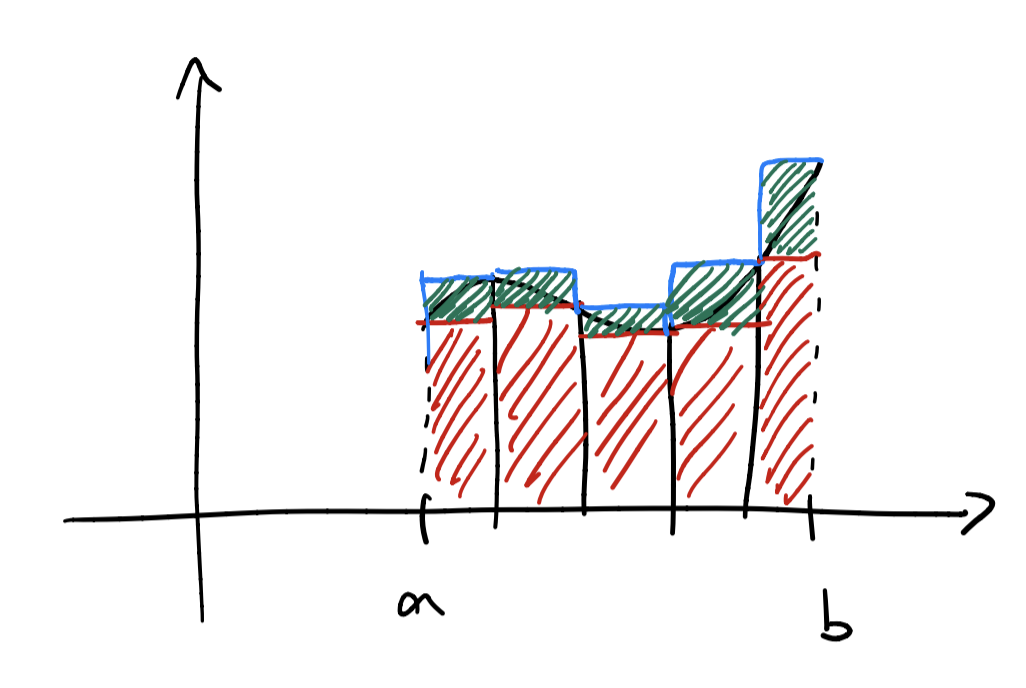
\includegraphics[width=4cm]{images/differenze-aree-integrale.png}
\end{wrapfigure}

Se $f$ è integrabile, $S''(f,A) - S'(f,A)$ (la differenza, l'area della regione verde nell'immagine) "tende a 0" al raffinarsi delle suddivisioni.
\vspace{15pt}
\subsection{Calcolo degli integrali}
\begin{theorem}
Siano $f,g$ integrabili su $[a,b]$ e un numero $k \in \mathbb{R}$, allora: $f+g, k\cdot, |f|$ sono integrabili, e si ha che:
\begin{enumerate}
    \item $\int_a^b (f+g)\:dx = \int_a^b f(x)\:dx + \int_a^b g(x)\:dx$.
    \item $\int_a^b (k\cdot f)\:dx = k \cdot \int_a^b f(x) \:dx$.
    \item Se $f(x) \leq g(x) \forall x \in [a,b]$ allora $\int_a^b f(x) \:dx \leq \int_a^b g(x)\:dx$.
    \item $\big|\int_a^b f(x) \:dx \big| \leq \int_a^b |f(x)|\:dx$.
    \item Se $a < c < b$ allora $\int_a^b f(x) \:dx = \int_a^c f(x) \:dx + \int_c^b f(x)\:dx$.
\end{enumerate}
\end{theorem}

\newpage
\begin{figure}[h!]
    \centering
    \begin{subfigure}{.3\textwidth}
        \centering
        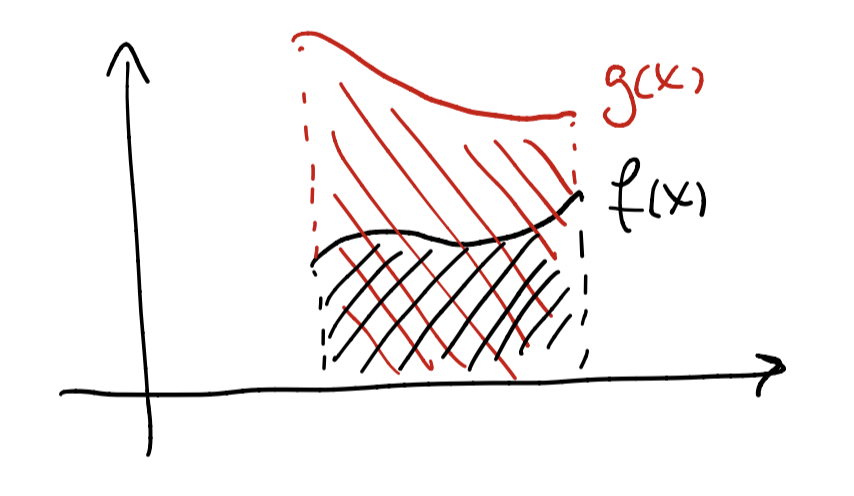
\includegraphics[width=4.5cm]{images/teorema-calcolo-integrali-1.png}
        \caption{Caso 1°}
    \end{subfigure}
    \begin{subfigure}{.3\textwidth}
        \centering
        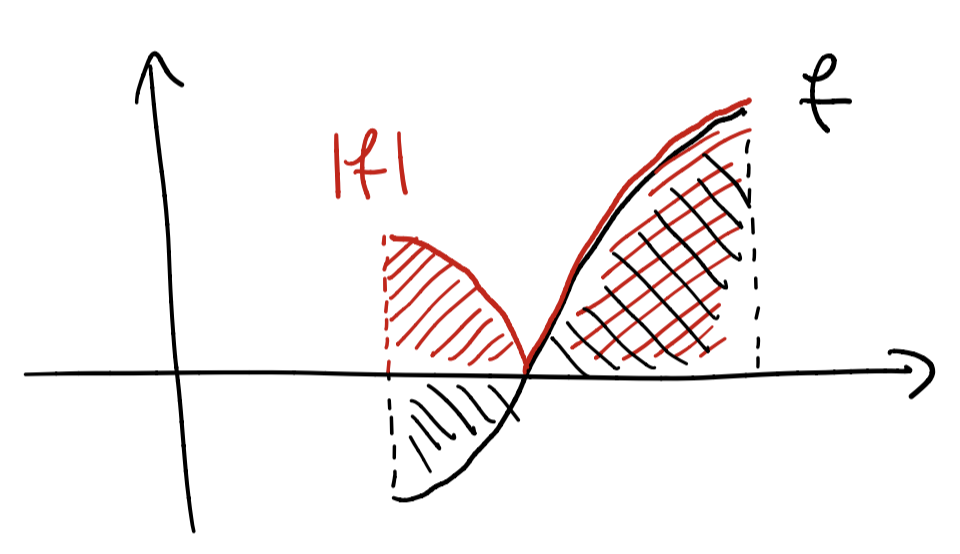
\includegraphics[width=4.5cm]{images/teorema-calcolo-integrali-2.png} 
        \caption{Caso 2°}
    \end{subfigure}
    \begin{subfigure}{.3\textwidth}
        \centering
        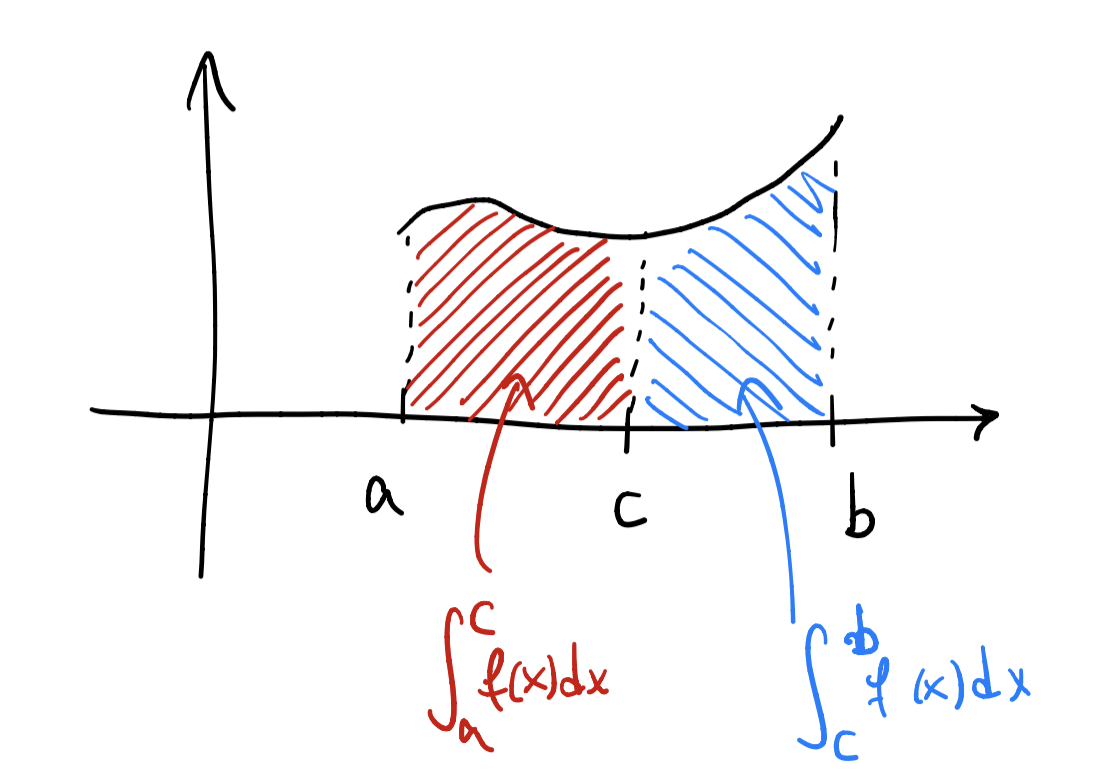
\includegraphics[width=4.5cm]{images/teorema-calcolo-integrali-3.png}
        \caption{Caso 3°}
    \end{subfigure}
\end{figure}

\begin{observation}
Osserviamo anche che se $f: [a,b] \to \mathbb{R}$ è constante, cioè $f(x) = k \:\: \forall x \in [a,b]$ allora $\int_a^b f(x) \:dx = k \cdot (b-a)$
\end{observation}

\subsection{Media Integrabile}
\begin{definition}[Media Integrabile]
Se $f: [a,b] \to \mathbb{R}$ integrabile, si dice \textbf{media integrabile} di $f$ su $[a,b]$.
\vspace{-10pt}
\[m = \frac{1}{b-a} \cdot \int_a^b f(x) \:dx\]\\
\end{definition}
\begin{wrapfigure}[2]{l}{5cm}
\vspace{-45pt}
    \centering
    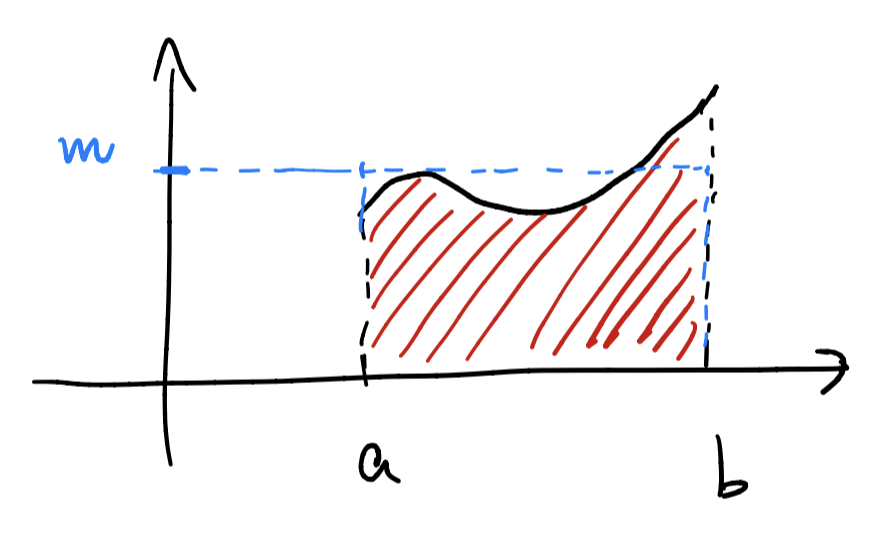
\includegraphics[width=4cm]{images/media-integrabile.png}
\end{wrapfigure}
\vspace{-10pt}
Graficamente, m è l'altezza di un rettangolo di base $b-a$, con la stessa area del sotto grafico di $f$.
\vspace{15pt}
\begin{theorem}[Teorema della media integrale]
Sia $f:[a,b] \to \mathbb{R}$ integrabile, allora:
\vspace{-5pt}
\[inf(f(x))_{[a,b]} \leq \frac{1}{b-a} \cdot \int_a^b f(x) \:dx \leq sup(f(x))_{[a,b]}\]
Se $f$ è continua, allora $\exists x \in [a,b]$ tale che:
$f(z) = \frac{1}{b-a} \cdot \int_a^b f(x) \:dx$
\end{theorem}

\begin{demostration}
$\forall x \in [a,b]$ abbiamo $inf(f(x))_{[a,b]} \leq f(x) \leq sup(f(x))_{[a,b]}$. Integriamo questa disuguaglianza usando la proprietà (3) del teorema, e otteniamo:\\
$\int_a^b inf(f(x))_{[a,b]}\:dx \leq \int_a^b f(x)\:dx \leq \int_a^b sup(f(x))_{[a,b]}\:dx$. Sia $\int_a^b inf(f(x))_{[a,b]}\:dx$ che $\int_a^b sup(f(x))_{[a,b]}\:dx$ sono costanti $\Longrightarrow \big( inf(f(x))_{[a,b]} \big)(b-a) \leq \int_a^b f(x)\:dx \leq \big( sup(f(x))_{[a,b]} \big)(b-a)$.\\
Dividendo per $(b-a)$ ottengo proprio: $inf(f(x))_{[a,b]} \leq \frac{1}{b-a} \cdot \int_a^b f(x) \:dx \leq sup(f(x))_{[a,b]}$.\\\\
Se $f$ è continua, allora per il teorema di Weirstrass $inf(f) = min(f)$ e $sup(f) = max(f)$. Inoltre per il teorema dei valor intermedi $f$ prende tutti i valori compresi tra il $min(x)$ e $max(f)$. La media integrale è un tale valore per quanto visto, quindi $\exists z \in [a,b]$ tale che $f(z) = \frac{1}{b-a} \cdot \int_a^b f(x)\:dx$. $\blacksquare$
\end{demostration}

\begin{observation}
Se $b<a$, definiamo $\int_a^b f(x)\:dx = - \int_b^a f(x)\:dx$, e definiamo anche $\int_a^a f(x) = 0$.
\end{observation}

\begin{example}
$\int_2^1 x^3\:dx = -\int_1^2 x^3\:dx$
\end{example}

\hspace{-15pt}Le proprietà viste precedentemente valgono anche con i valori scambiati come nell'esempio sopra.
\begin{observation}
La media integrale ha senso anche quando gli estremi sono scambiati. Se $b < a$, allora $\frac{1}{b-a}\int_a^b f(x)\:dx = (\frac{1}{b-a})\big(-\int_a^b f(x)\:dx \big) = \frac{1}{a-b}\int_a^bf(x)\:dx$
\end{observation}

\begin{definition}[Primitiva]
Prendiamo un $I\subseteq \mathbb{R}$ intervallo, $f: I \to \mathbb{R}$, una funzione $F: I \to \mathbb{R}$ si dice primitiva di $f$ se $F$ è derivabile in $I$ e vale che $F'(x) = f(x) \:\: \forall x \in I$.
\end{definition}

\begin{example}
$f(x) = 2x$. Una primitiva è $F(x) = x^2$. Non è l'unica primitiva, $G(x) = x^2 + k$, $k\in \mathbb{R}$ ho comunque $G'(x) = 2x + 0 = f(x)$ quindi queste funzioni sono tutte primitive di $f(x) = 2x$. 
\end{example}
\hspace{-15pt}In generale, se $F$ è primitiva di $f$, tutte le funzioni $G(x) = F(x) + k$ con $k \in \mathbb{R}$ sono pure primitive di $f(x)$.

\begin{observation}
In effetti due primitive di $f(x)$ differiscono sempre per una costante.
\end{observation}

\begin{demostration}
Siano F e G due primitive di $f$. Allora ho che $F' = f$, $G' = f$. Quindi $(F - G)' = F' - G' = f - f = 0$. Visto che siamo su un intervallo, concludo che $F - G$ è costante $K \in \mathbb{R} \Longrightarrow F(x) = G(x) + k \:\: \forall x \in I$.
\end{demostration}

\begin{definition}[Integrale indefinito]
\textbf{L'integrale indefinito} di $f(x)$ è l'insieme di tutte le primitive di $f(x)$ e si indica con $\int f(x)\:dx$ (senza gli estremi).
\end{definition}

\begin{observation}
$\int f(x)\:dx$ non indica una singola funzione, ma un insieme di funzioni.
\[\int f(x)\:dx = \{F: I \to \mathbb{R} \:\: | \:\: F \: derivabile \: e \: F'=f\}\]
\end{observation}

\begin{example}
Se prendiamo per esempio $\int 2x\:dx = \{x^2 + k \:\:|\:\: k \in \mathbb{R}\}$ di solito si abbrevia scrivendo $\int 2x\:dx = x^2 + k$. 
\end{example}

\hspace{-15pt}L'integrale di Riemainn $\int_a^b f(x)\:dx$ invece è un numero reale, e rappresenta l'area del sotto grafico di $f$, e si dice \textbf{integrale definito} e $a,b$ sono gli \textbf{estremi di integrazione} ("a" è inferiore e "b" superiore). 

\subsection{Formule per integrali indefiniti}
Dalle formule per le derivate seguono formule per le primitive di una funzione f(x). Vedere la tabella di seguito.
\begin{table}[h!]
    \centering
    \setlength{\tabcolsep}{6pt}
    \renewcommand{\arraystretch}{1.5}
    \begin{tabular}{|c||c|}
        \hline
        $\int e^x=e^x + k$ & $\int \frac{1}{x}\:dx=\log|x| + k$\\
        
        $\int \cos(x)\:dx=\sin{x} + k$ & $\int \sin{x}\:dx=-\cos(x) + k$ \\
        
        $\int \frac{1}{1+x^2}\:dx=\arctan{x} + k$ & $\int \frac{1}{\sqrt{1 - x^2}}\:dx=\arcsin{x}$\\
        
        $\int \frac{1}{(\sin{x})^2}\:dx=-\cot{x}$ & $\int \frac{1}{(\cos{x})^2}\:dx=\tan{x}$ \\
        
        $\int x^n \:dx=\frac{1}{n+1}x^{n+1} + k$ & $\int -\frac{1}{x^2}\:dx=\frac{1}{x}$\\
        \hline
    \end{tabular}
    \caption{Formule primitive}
\end{table}
\vspace{-10pt}
\subsection{Teorema fondamentale del calcolo integrale}
\begin{theorem}[Teorema fondamentale del calcolo integrale]
Sia $I \subseteq \mathbb{R}$ un intervallo, $a \in I$, $f: I \to \mathbb{R}$ continua. Allora la funzione $F(x) = \inf_a^x f(t) \:dt$ (chiamata anche funzione integrale) è una primitiva di $f$, cioè $F(x)$ è derivabile e $F'(x) = f(x)$.
\end{theorem}

\begin{demostration}
Mostriamo che $F$ è derivabile calcolandone il rapporto incrementale in $x_0 \in I$ arbitrario, e poi facendo il limite.\\\\
$\frac{F(x) - F(x_0)}{x - x_0} = \frac{1}{x - x_0}\big( \int_a^x f(y) \:dt - \int_a^{x_0} f(y) \:dt \big) = \frac{1}{x - x_0} \int_{x_0}^x f(t) \:dt$. In risultato è la media integrale di $f$ sull'intervallo di estremi $x$ e $x_0$.\\\\
Visto che $f$ è continua, per il teorema della media integrale $\exists \: z(x)$ compreso tra $x_0$ e $x$ tale che $f(z(x)) = \frac{1}{x - x_0} \int_{x_0}^x f(t) \:dt$.\\
Quindi $F'(x_0) = \lim\limits_{x\to x_0}\frac{F(x) - F(x_0)}{x - x_0} = \lim\limits_{x\to x_0}f(z(x))$. Cambio variabile e prendo $y = z(x)$. Devo capire a cosa tende $y$ quando $x\to x_0$. So che $z(x)$ è compreso tra $x_0$ e $x$ (ad esempio se $x \leq x_0$, so che $x \leq z(x) \leq x_0$) quindi per il teorema dei carabinieri ho che $\lim\limits_{cx \to x_0}y = x_0$.\\\\
Segue che $\lim\limits_{x \to x_0}f(z(x)) = \lim\limits_{y \to x_0} f(y) = f(x_0)$ (questo per la continuità di f). Questo dimostra che $F'(x_0) = f(x_0)$m quindi $F'(x) = f(x) \:\: \forall x \in I$. $\blacksquare$
\end{demostration}

\newpage
\subsection{Teorema di Torricelli}
\begin{theorem}[Teorema di Torricelli]
$I \subseteq \mathbb{R}$ intervallo, $f: I \to \mathbb{R}$ funzione continua, $a \in I$. Se G è una primitiva di $f$ in I, allora $\exists k \in \mathbb{R}$ tale che $G(x) = \int_a^x f(t) \:dt + k$ e $\forall \alpha, \beta \in I$ abbiamo che $\int_{\alpha}^{\beta}f(t) \:dt = G(\beta) - G(\alpha)$.
\end{theorem}

\hspace{-15pt}A livello di notazioni si va a scrivere: $[G(x)]_{\alpha}^{\beta} = G(\beta) - G(\alpha)$

\begin{example}
Prendiamo $\int_1^3 x \:dx$. Una primitiva di $f(x) = x$ è $G(x) = \frac{x^2}{2}$. \\
Quindi $\int_1^3 x \:dx = [\frac{x^2}{2}]_1^3 = \frac{9}{2} - \frac{1}{2} = \frac{8}{2} = 4$. (Se prendiamo un'altra primitiva ad esempio $F(x) = \frac{x^2}{2} + 1$, trovato $\int_1^3 x \:dx = [\frac{x^2}{2} + 1]_1^3 = \frac{8}{2} = 4$)
\end{example}

\subsection{Integrali con estremi variabili}
\begin{theorem}
Dato un $I \subseteq \mathbb{R}$ intervallo, $f: I \to \mathbb{R}$ continua. Abbiamo poi $A\subseteq \mathbb{R}$, e $\alpha,\beta:A \to I$ derivabili. Sia $G(x) = \int_{\alpha(x)}^{\beta(x)} f(t) \:dt$. Allora $G(x)$ è derivabile e si ha:
\[G'(x) = f(\beta(x)) \cdot \beta'(x) - f(\alpha(x)) \cdot \alpha'(x)\]
In particolare se $\alpha(x) = a$ constante e $\beta(x) = x$, si ha $G(x) = \int_a^x f(t)\:dt$, e la formula scritta sopra è uguale a $f(x) \cdot \ - f(a) \cdot 0 = f(x)$. (Come della conclusione del teorema fondamentale)
\end{theorem}

\begin{example}
$G(x) = \int_{x^2}^{\sin{x}}e^t \cdot \arctan(t) \:dt$ \hfill $f(t) = e^t \arctan(t)$, $\alpha(x) = x^2$, $\beta(x) = \sin(x)$.\\
Abbiamo $G'(x) = f(\beta(x)) \cdot \beta'(x) - f(\alpha(x)) \cdot \alpha'(x) = e^{\sin{x}} \cdot \arctan(\sin(x)) \cdot \cos(x) - e^{x^2} \cdot \arctan(x^2) \cdot 2$.\\
Applicazione: $\lim\limits_{x\to 0}\frac{\int_0^{x^2} e^t \cdot \arctan(x) \:dt}{\sin(x^4)} = \frac{\int_0^0 (...)}{\sin(0)} = \frac{0}{0}$. Usiamo de l'hopital.\\
$\lim\limits_{x\to 0} \frac{e^{x^2}\cdot \arctan(x^2) \cdot 2x}{\cos(x^4) \cdot 4x^3} = \lim\limits_{x\to 0}\frac{e^{x^2}}{\cos(x^4)}\cdot\frac{\arctan(x^2) \cdot x}{2x^3} = \lim\limits_{x\to 0} \frac{e^{x^2}}{\cos(x^4)}\cdot \frac{\arctan(x^2)}{2x^2} = \lim\limits_{x\to 0}\frac{e^{x^2}}{\cos(x^4)}\cdot\frac{x^2 + o(x^2)}{2x^2} = 1 \cdot \frac{1}{2}$
\end{example}

\subsection{Metodi di calcolo per integrali indefiniti}
\subsubsection{Integrazione per parti}
Prendiamo $f,g: I \to \mathbb{R}$ con $I\subseteq \mathbb{R}$ intervallo, $f$ continua e $g$ di classe $C^1$ ($g$ e derivabile e la derivata è continua). Se $F$ è una primitiva di $f$ allora:
\vspace{-5pt}
\[\int f\cdot g\:dx = F \cdot g - \int F \cdot g' \:dx\]

\begin{demostration}
Se faccio la derivata del prodotto $(F \cdot g)' = F'\cdot g + F\cdot g' = fg + F'g$. \\
(Se due funzioni sono uguali anche gli integrali indefiniti delle due funzioni sono uguali)Integrando ambo i membri ottengo che $\int (Fg)'\:dx = \int (fg)\:dx + \int F\cdot g' \:dx = \int F\cdot g\:dx = \int (fg)\:dx + \int F\cdot g' \:dx$. Abbiamo così dimostrato la formula. $\blacksquare$
\end{demostration}

\hspace{-15pt}Esempi ed esercizi guarda i lucidi delle lezioni (gli appunti del professore).

\begin{observation}
Se il ho $\log(f(x))' = \frac{f'(x)}{f(x)}$ (sto supponendo che $f(x) > 0$), quindi segue che $\int \frac{f'(x)}{f(x)} \:dx = \log(f(x)) + k$.
\end{observation}

\subsubsection{Integrazione per sostituzione}
Supponiamo di avere $I,J \subseteq \mathbb{R}$ intervalli, $f: I \to \mathbb{R}$ continua. Prendiamo poi $\phi: J \to I$ di classe $C^1$. Se $F$ è una primitiva di $f$, allora $\int (f \circ \phi) \cdot \phi' \:dx = (F \circ \phi) + k$.

\begin{demostration}
$(F \circ \phi)' = (F'(\phi)) \cdot \phi' = (f \circ \phi) \cdot \phi'$ per la regola di derivazione di funzioni composte, Integrando trovo che: $\int (f \circ \phi) \cdot \phi' \: dx = \int (F \circ \phi)' \:dx = (F \circ \phi) + k$. $\blacksquare$
\end{demostration}

\begin{example}
Prendiamo $\int xe^{x^2}\:dx$. Pongo $t=x^2$ (funzione di x), $\frac{dt}{dx} = dx$ quindi $dt = 2xdx$, $\frac{dt}{2} = xdx$.\\
$\int e^t \cdot \frac{dt}{2} = \frac{1}{2}\int e^t \:dt = \frac{1}{2} e^t +c$ e poi si torna in $x$ sostituendo $t=x^2$ quindi torna $\frac{1}{2}e^{x^2} + k$.\\\\
Per gli integrali definiti possiamo fare in due modi. Prendiamo $\int_0^2 xe^{x^2}\:dx$:
\begin{enumerate}
    \item Calcolare $\int xe^{x^2}\:dx$. Abbiamo che che è $\frac{1}{2}e^{x^2} + k$. Poi $\int_0^2 xe^{x^2}\:dx = [\frac{1}{2}e^{x^2} + k]_0^2 = \frac{1}{2}(e^4-1)$.
    \item Possiamo usare la sostituzione, ricordandosi di cambiare gli estremi: $\int_0^2 xe^{x^2}\:dx$ pongo come prima  $dt = 2xdx$, $\frac{dt}{2} = xdx$.\\
    Quindi $\int_0^2 xe^{x^2}\:dx = \int \frac{e^t}{2}\:dt$ e bisogna calcolare gli estremi vedendo quanto vale t negli estremi.\\
    $x= 0$ quindi $t = 0^2 = 0$ e $x = 2$ quindi $t = 2^2 = 4$. Alla fine avremo  $\int_0^4 xe^{x^2}\:dx$, da qui poi si va avanti come prima.
\end{enumerate}
\end{example}

\begin{example}
$\int \sqrt{1-x^2}\:dx$. $x = \sin(t)$, $t = \arcsin(x)$ e $\frac{dx}{dt} = \cos(t)$ quidi $dx = \cos(t) \:dt$.\\
$= \int \sqrt{1-\sin(t)^2} \cdot \cos(t) \:dt = \int \sqrt{\cos(t)^2} \cdot \cos(t) \:dt = \int |\cos(t)| \cdot \cos(t) \:dt$ (il valore assoluto si toglie visto che $\cos(t) \geq 0$ nell'intervallo in cui stiamo integrando che è fra $-\frac{\pi}{2}$ e $\frac{\pi}{2}$).\\
$\int \cos(t)^2 \:dt = \frac{t + \sin(t)\cdot\cos(t)}{2} + c = \frac{\arcsin(x) + x \cdot \sqrt{1 - x^2}}{2} + c$.
\end{example}

\hspace{-15pt}Se andiamo a fare l'integrale di $f(x) = \sqrt{1-x^2}$ si va a calcolare l'area del cerchio unitario.\\
Infatti $4 \int_0^1 \sqrt{1-x^2}\:dx = 4\big[\frac{\arcsin(x) + x\sqrt{1-x^2}}{2}\big]_0^1 = 4 \cdot \frac{\arcsin(1)}{2} = 2 \frac{\pi}{2} = \pi$.\\\\
Se volessimo calcolare $\int \frac{1}{\sqrt{1 - x^2}}\:dx = \arcsin(x) + k$ visto che $(\arcsin(x))' = \frac{1}{\sqrt{1 - x^2}}$.
\begin{observation}
Ho anche $(\arccos(x))' = -\frac{1}{\sqrt{1-x^2}}$, quindi $\int \frac{1}{\sqrt{1-x^2}}\:dx = -\int -\frac{1}{\sqrt{1-x^2}}\:dx = -\arccos(x) + k'$. Segue che $\arcsin(x) - (-\arccos(x))$ è costante. Per vedere quanto vale basta calcolare in $x=0$, e trovo $\arcsin(0) + \arccos(0) = 0 + \frac{\pi}{2}$. Quindi  $\arcsin(x) + \arccos(x) = \frac{\pi}{2} \:\: \forall x \in [-1,1]$.
\end{observation}

\subsection{Integrali di funzioni razionali}
Consideriamo integrali nella forma $\int \frac{p(x)}{q(x)} \:dx$ dove $p(x)$ e $q(x)$ sono polinomi in x ed il grado di $q(x) \leq 2$, $\deg(q(x)) \leq 2$.
\begin{itemize}
    \item Caso con denominatore ha grado 1, $\deg(q(x)) = 1$.\\
    Esempio caso particolare con numeratore costante con $\int \frac{1}{ax + b}\:dx$. In questo caso usiamo la sostituzione $y = ax+b$ e $dy = a \cdot dx$.\\
    $= \int \frac{1}{y} \cdot \frac{dy}{a} = \frac{1}{a} \int \frac{1}{y}\:dy = \frac{1}{a} \log|ax+b| + c$.\\\\
    Caso con $\deg(p(x)) > 0$. Usiamo il caso precedente ma facendo prima la divisione di polinomi di $p(x)$ per $q(x) = ax + b$. Cioè scriviamo:\\
    $p(x) = (ax + b) \cdot Q(x) + R(x)$ dove $Q(x)$ e $R(x)$ sono polinomi e $\deg R(x) < \deg(ax + b) = 1$, (allora R(x) è una costante ed è uguale a $p(-\frac{b}{a})$).\\\\
    C'è un algoritmo per fare la divisione in maniera veloce:
    \begin{example}
    Prendiamo $\int \frac{2x^2 + 1}{x+1}\:dx$. $\frac{p(x)}{ax + b} = \frac{2x^2 +1}{x+1}$, quindi $a=1$ e $b=1$.\\
    Divido $2x^2 + 1$ per $x+1$. (Fare la divisione, vedere gli appunti delle lezioni per il modo preciso).\\
    Il risultato è: $\int \frac{(x+1)(2x-2)+3}{x+1}\:dx = \int \frac{(x+1)(2x-2)}{(x+1)}dx + \int \frac{3}{x+1} = \int (2x-2)dx + 3\log|x+1| + c = x^2 -2x + 3\log|x+1| + c$
    \end{example}
    
    \item Caso con grado denominatore uguale a 2, $\deg(q(x)) = 2$.\\
    Il primo passaggio è sempre quello di fare la divisione scrivendo $p(x) = (ax^2 + bx + c) \cdot Q(x) + R(x)$ dove $\deg R(x) <2$ cioè $R(x) = cx + d$.\\
    Quindi $\int \frac{p(x)}{q(x)}dx = \int \frac{(ax^2 + bx + c) \cdot Q(x) + R(x)}{ax^2 + bx + c} dx = \int Q(x)dx + \int \frac{R(x)}{ax^2 + bx + c}dx$, dove $R(x) = cx+d$.\\
    Per calcolare gli integrali di questa forma rimane da vedere come calcare $\int \frac{cx + d}{ax^2 + bx + c}dx$.\\
    Ci sono usa serie di casi particolare da analizzare, a seconda del numero di radici reali del denominatore:
    \begin{enumerate}
        \item Due radici coincidenti e numeratore costante. $\int \frac{dx}{(x-a)^2}$, si fa una sostituzione del tipo $y= x-a$ e $dy= dx$.
        $\int \frac{dy}{y^2} = \int y^{-2}\:dy = \frac{1}{-1} \cdot y^{-1}+c = -\frac{1}{y} + c = -\frac{1}{x-a} + c$.
        \item Due radici reali distinte e numeratore costante. $\int \frac{dx}{(x-a)(x-b)}$ con $a\neq b$. Si cercano due numeri reali A e B tali che valga:\\
        $\frac{1}{(x-a)(x-b)} = \frac{A}{(x-a)} + \frac{B}{(x-b)} = \frac{A(x-b) + B(x-a)}{(x-a)(x-b)} = \frac{x(A+B) - Ab - Ba}{(x-a)(x-b)}$. Se voglio che valga questa uguaglianza, per il principio di identità dei polinomi deve essere che:\\\\
        $\begin{cases}A+B=0\\-Ab-Ba = 1\end{cases}=$\hspace{.3cm}$\begin{cases}B = -A\\-Ab + Aa = 1\end{cases}=$\hspace{.3cm}$\begin{cases}A+B=0\\A=\frac{1}{a-b}\end{cases}=$\hspace{.3cm} $\begin{cases}B = -\frac{1}{a-b}\\A=\frac{1}{a-b}\end{cases}$\\\\
        A questo punto posso sostituire con l'espressione trovata sopra:\\
        $\int \frac{dx}{(x-a)(x-b)} = \int (\frac{1}{a-b} \cdot \frac{1}{(x-a)} - \frac{1}{a-b}\cdot\frac{1}{(x-b)})dx = \frac{1}{a-b} (\log|x-a) - \log|x-b|) + c$
    \end{enumerate}
    
    \item Denominatore senza radici reali e numeratore costante.\\
    $\int \frac{dx}{1+x^2}dx = \arctan(x) + c$. Generalizzando $\int \frac{dx}{k^2 + x^2}$ con $k \in \mathbb{R}$ e $k\neq 0$.\\
    $\int \frac{dx}{k^2 + x^2} = \frac{1}{k^2}\cdot \int \frac{dx}{1 + (\frac{x}{k})^2}$ facciamo poi una sostituzione con $y= \frac{x}{k}$ e $dy = \frac{dx}{k}$.\\
    $\frac{1}{k^2} \int \frac{1}{a+y^2} \cdot k \: dy = \frac{1}{k} \cdot \arctan(y) + c = \frac{1}{k} \cdot \arctan(\frac{x}{k}) + c$.\\
    Il casi generale con il denominatore come $ax?2 +bx + c$ senza radici reali, cioè $\Delta < 0$. In realtà posso supporre che $a = 1$:
    $\int \frac{1}{ax^2 + bx + c}dx = \frac{1}{a}\cdot \int \frac{1}{x^2 + \frac{b}{a}x + \frac{c}{a}}dx$. Quindi guardo polinomi della forma $x^2 + bx + c$ con $\Delta < 0$. Io posso fare $x^2 + bx + c = (x^2 + bx + \frac{b^2}{4}) - \frac{b^2}{4} + c = (x + \frac{b}{2})^2 + \frac{1}{4}(-b^2 + 4c)$.\\
    $\int \frac{dx}{x^2 + x + c} = \int \frac{dx}{(x + \frac{b}{2})^2 + k^2}$, con $k^2 = \frac{1}{4}(-b^2 + 4c) > 0$. Se poi andiamo a sostituire con $y = x + \frac{b}{2}$ e $dy = dx$ abbiamo $\int \frac{1}{y^2 + k^2}dx$ e questo lo sappiamo fare perché visto sopra ed è $\frac{1}{k}\arctan(\frac{x + \frac{b}{2}}{k})+c$.
    
    \begin{example}
    $\int \frac{dx}{x^2 + 2x + 10} = \int \frac{dx}{x^2 + 2x + 1 - 1 + 10} = \int \frac{dx}{(x+1)^2 + 9} = \int \frac{dy}{y^2 + 9} = \frac{1}{3}\arctan(\frac{x+1}{3})+c$.\\
    (se si fosse scelto $k=-3$ invece che $k=3$ sarebbe venuto lo stesso risultato perché $-\frac{1}{3}\arctan(-\frac{y}{3}) + c = \frac{1}{3}\arctan(\frac{y}{3})$)
    \end{example}
    
    \item Caso nel quale il denominatore non è costante, cioè ha grado 1, bisogna vedere come comportarsi con il numeratore.\\
    $\int \frac{ax + b}{x^2 + cx + d}dx = \frac{a}{2} \int \frac{2x + \frac{2b}{a}}{x^2 + cx + d}dx = \frac{a}{2}\int \frac{2x + c - c + \frac{2b}{a}}{x^2 + cx + d} = \frac{a}{2}\int \frac{2x + c}{x^2 + cx + d}dx + \frac{a}{2}\int \frac{-c \frac{2b}{a}}{x^2 + cx + d}dx$ ora per il primo integrale il numeratore è la derivata del denominatore, mentre nel secondo essendoci una costante al numeratore lo sappiamo fare.\\
    $\frac{a}{2}\log|x^2 + cx + d| + \frac{a}{2}\int \frac{-c + \frac{2b}{a}}{x^2 + cx + d}dx$.
    \begin{example}
    $\int \frac{4x + 5}{x^2 + 2x - 1}dx = 2\int \frac{2x + \frac{5}{2} + 2 - 2}{x^2 + 2x - 1}dx = 2 \int \frac{2x + 2}{x^2 + 2x - 1}dx + 2 \int \frac{\frac{1}{2}}{x^2 + 2x - 1}dx =$\\ $=2\log|x^2 + 2x - 1| + \int \frac{1}{x^2 + 2x - 1}$
    \end{example}
\end{itemize}

\subsection{Integrali impropri}
Gli Integrali impropri o generalizzati estendono la definizione di integrale definito al caso in cui l'integrale non è limitato, oppure l'intervallo di integrazione non è limitato.
\begin{example}
Dobbiamo dare un senso per esempio a $\int_0^{+\infty}e^{-x}\:dx$.
\end{example}
\begin{wrapfigure}[6]{r}{5cm}
    \vspace{-25pt}
    \centering
    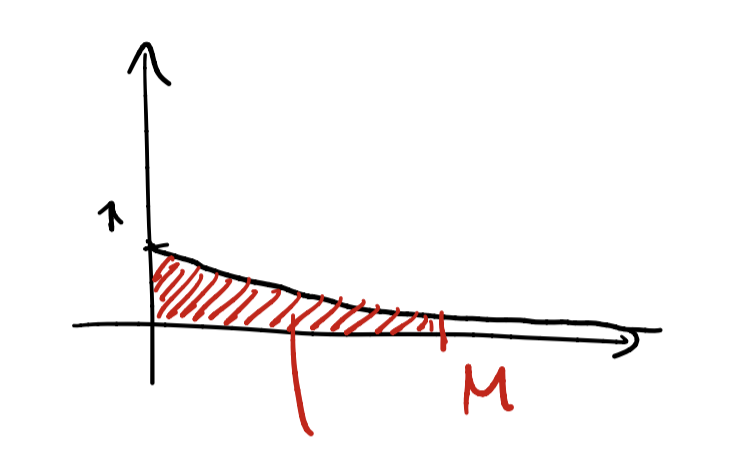
\includegraphics[width=4.5cm]{images/esempio-integrale-improprio-1.png}
\end{wrapfigure}
Intuitivamente rappresenta l'area di tutto il sotto grafico sopra $(0,+\infty)$.
Formalmente definiremo un limite: \\\\
$\lim\limits_{M\to +\infty}\int_0^Me^{-x}\:dx = \lim\limits_{M\to + \infty}[-e^{-x}]^M_0=\lim\limits_{M\to +\infty}-e^{-M}+1 = 1$.\\
In questo caso il sotto grafico $[0,+\infty)$ ha area finita uguale a 1.

\begin{example}
Se invece prendiamo $\int_0^{+\infty}\frac{1}{1+x}dx = \lim\limits_{M\to +\infty}\int_0^{M}\frac{1}{1+x}dx = \lim\limits_{M\to +\infty}[\log(1+x)]_0^M = \lim\limits_{M\to +\infty}(\log(1+M)-0) = +\infty$. In questo caso l'area del sotto grafico è infinito.
\end{example}
\newpage
\begin{example}
Facciamo un' altro esempio di integrale improprio con $\int_0^1 \frac{1}{\sqrt{x}}dx$.
\end{example}
\begin{wrapfigure}[5]{l}{4.5cm}
    \vspace{-25pt}
    \centering
    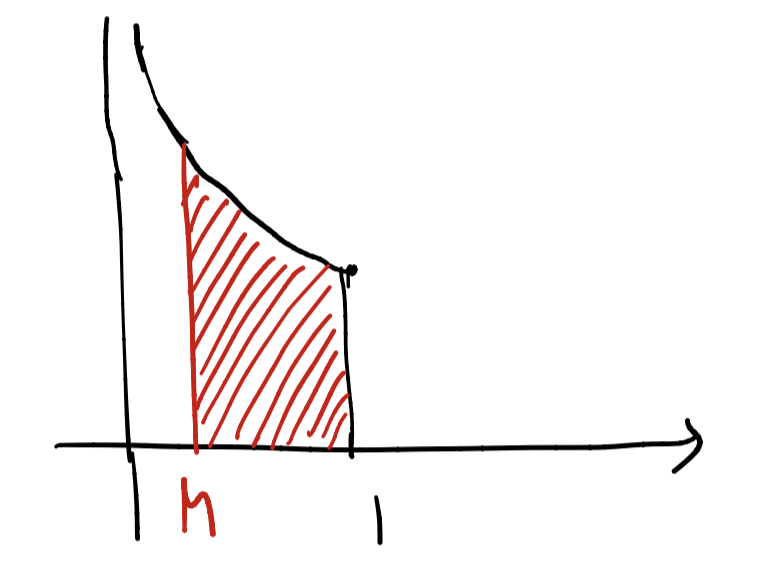
\includegraphics[width=3.7cm]{images/esempio-intergale-improprio-2.png}
\end{wrapfigure}
$\int_0^1 \frac{1}{\sqrt{x}}dx$ notiamo che la funzione $\frac{1}{\sqrt{x}}$ non è limitata sull'intervallo compreso fra $[0,1)$.\\\\
$\lim\limits_{M\to 0^+}\int_M^1 \frac{1}{\sqrt{x}}dx = \lim\limits_{M\to 0^+}[2\sqrt{x}]_M^1 = \lim\limits_{M\to 0^+}(2-2\sqrt{M}) = 2$, l'area del sotto grafico di $\frac{1}{\sqrt{x}}$ sopra a $[0,1]$.
\vspace{10pt}
\begin{example}
$\int_0^1 \frac{1}{x}dx = \lim\limits_{M\to 0^+}\int_0^1 \frac{1}{x}dx = \lim\limits_{M\to 0^+}[\log(x)]_M^1 = \lim\limits_{M\to 0^+} (0-\log(M)) = + \infty$.\\
Quindi in questo caso il sotto grafico ha area infinita.
\end{example}
\begin{definition}[Integrali impropri o generalizzati]
Dati due punti $a\in \mathbb{R}$ e $b \in \mathbb{\overline{R}}$, $a<b$ e $f:[a,b)\to \mathbb{R}$ che sia integrabile in tutti gli intervalli $[a,M]$ con $a<M<b$. Se esiste $\lim\limits_{M\to b^-}\int_a^M f(x)\:dx = L$, definiamo $\int_a^b f(x)\:dx = L$. 
\begin{itemize}
    \item Se L è reale finito si dice che l'integrale di $f(x)$ su $[a,b)$ converge (oppure che $f(x)$ è integrabile "in senso generalizzato su $[a,b)$").
    \item Se L è uguale a $+\infty$ si dice che l'integrale diverge positivamente (o "a $+\infty$").
    \item Se L è uguale a $-\infty$ si dice che l'integrale diverge negativamente (o "a $-\infty$").
\end{itemize}
\end{definition}
\hspace{-15pt}Vedendo gli esempi visti sopra possiamo dire che:\\
$\int_0^{+\infty}e^{-x}\:dx$ converge \hfill $\int_0^{+\infty}\frac{1}{1+x}\:dx$ diverge pos. \hfill $\int_0^1 \frac{1}{\sqrt{x}}\:dx$ converge \hfill $\int_0^1\frac{1}{x}\:dx$ diverge pos.

\begin{example}
Esempio in cui il limite non esiste: 
\end{example}
\begin{wrapfigure}[2]{l}{4.5cm}
    \vspace{-25pt}
    \centering
    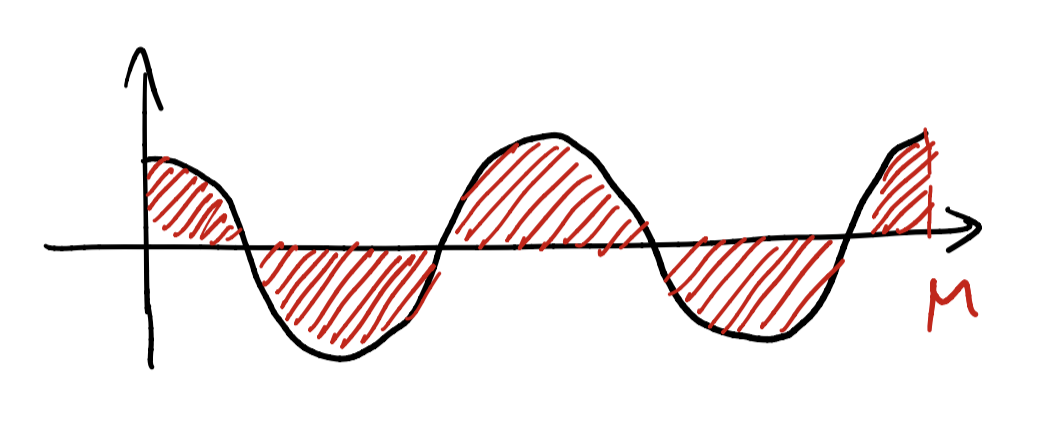
\includegraphics[width=4cm]{images/esempio-integrale-improprio-3.png}
\end{wrapfigure}
$\int_0^{+\infty}\cos(x)\:dx = \lim\limits_{M\to +\infty}\int_0^M\cos(x)\:dx = \lim\limits_{M\to +\infty}[\sin(x)]_0^M = \lim\limits_{M\to +\infty}(\sin(M)-0)$ e questo non esiste.\\\\

\hspace{-15pt}Analogamente si definisce $\int_a^b f(x)\:dx$ quando $f:(a,b] \to \mathbb{R}$ con $a \in \mathbb{\overline{R}}$, $b\in \mathbb{R}$ e $f$ integrabile su $[M,B] \forall a < M < b$ come $\lim\limits_{M\to a^+}\in_M^b f(x) \:dx$ (se esiste).\\\\
Se però abbiamo $f:(a,b)\to \mathbb{R}$ questa funzione "ha un problema" in entrambi a e b, ad esempio $\int_{-\infty}^{+\infty}\frac{1}{1+x^2}\:dx$ oppure $\int_{-1}^1 \frac{1}{1-x^2}\:dx$.

\begin{definition}
Sia $f: (a,b)\to \mathbb{R}$ con $a,b \in \mathbb{\overline{R}}$ che sia integrabile su $[M_1,M_2]$ con $a<M_1<M_2<b$. Scegliamo arbitrariamente $c\in (a,b)$, se esistono entrambi $\int_a^c f(x)\:dx$ e $\int_c^b f(x)\:dx$ allora si definisce:
\[\int_a^b f(x)\:dx = \int_a^c f(x)\:dx + \int_c^b f(x)\:dx \text{ Se la somma non è indeterminata (cioè non è} +\infty-\infty)\]
E in questo caso si diche che $f$ è integrabile in senso improprio su (a,b)
\end{definition}

\begin{observation}
L'esistenza e il valore di $\int_a^b f(x) \:dx$ non dipende dalla scelta di $c\in (a,b)$.\\
Se scelgo $d\in (a,b)$ ho $\int_a^b f(x)\:dx = \int_a^c f(x)\:dx + \int_c^b f(x)\:dx$ e $\int_d^b f(x)\:dx = \int_d^c f(x)\:dx + \int_c^b f(x)\:dx$.\\
Sommando queste due equazioni ottengo $\int_a^b f(x)\:dx + \int_d^b f(x)\:dx = \int_a^c f(x)\:dx + \int_c^b f(x)\:dx + \int_c^d f(x)\:dx + \int_d^c f(x)\:dx$ la seconda somma $\int_c^d f(x)\:dx + \int_d^c f(x)\:dx = 0$ quindi vediamo che il risultato non cambia.
\end{observation}

\begin{example}
$\int_{-\infty}^{+\infty} \frac{1}{1+x^2}\:dx$. Scelgo $c=0$.\\
$\int_{-\infty}^0 \frac{1}{1+x^2}\:dx = \lim\limits_{M\to -\infty} \int_M^0\frac{1}{1+x^2}\:dx = \lim\limits_{M\to -\infty} [\arctan(x)]_{-M}^0 = \lim\limits_{M\to -\infty}[0 -\arctan(M)] = +\frac{\pi}{2}$\\\\
$\int_0^{+\infty}\frac{1}{1+x^2}=$ (stessi conti di prima) $= \frac{\pi}{2}$.
Quindi $\int_{-\infty}^{+\infty}\frac{1}{1+x^2}\:dx = \frac{\pi}{2}+\frac{\pi}{2} = 2$ (converge)
\end{example}

\begin{example}
$\int_0^{+\infty}\frac{1}{x^2}dx$, scegliamo $c=1$.\\
$\int_0^1 \frac{1}{x^2}\:dx = \lim\limits_{M\to 0^+} \int_M^1\frac{1}{x^2}\:dx = \lim\limits_{M\to 0^+}[-x^{-1}]_M^1 = \lim\limits_{M\to 0^+}[-1+\frac{1}{M}]_M^1 = +\infty$ (diverge positivamente).\\
$\int_1^{+\infty}\frac{1}{x^2}\:dx = \lim\limits_{M\to +\infty}\int_1^M \frac{1}{x^2}\:dx = \lim\limits_{M\to +\infty}[-x^{-1}]_1^M = \lim\limits_{M\to +\infty}[-\frac{1}{M} + 1] = 1$.\\
Quindi $\int_0^+\infty \frac{1}{x^2}\:dx = +\infty + 1 = +\infty$ quindi il grafico diverge positivamente.
\end{example}

\begin{example}
Prendiamo $\int_{-1}^1 \frac{1}{x}\:dx$ in questo caso spezziamo in $c=0$.\\
$\int_{-1}^1 \frac{1}{x}dx = \int_{-1}^0 \frac{1}{x}\:dx + \int_0^1\frac{1}{x}\:dx$.\\
$\int_{-1}^0 \frac{1}{x}\:dx = \lim\limits_{M\to 0^-}\int_{-1}^M =  \lim\limits_{M\to 0^-} [\log(-x)]_{-1}^M =  \lim\limits_{M\to 0^-} \log(-M) = -\infty$.\\
$\int_0^1\frac{1}{x}\:dx = \lim\limits_{M\to 0^+}\int_M^1\frac{1}{x}\:dx = \lim\limits_{M\to 0^+} [\log(x)]_M^1 = \lim\limits_{M\to 0^+} -\log(M) = +\infty$.\\
Se vado a fare la soma ho che la somma è indeterminata $\int_{-1}^1 \frac{1}{x}\:dx = +\infty - \infty$ e dunque non esiste.\\\\
Attenzione a non fare $\int_{-1}^1 \frac{1}{x}\:dx = [\log|x|]_{-1}^1 = \log(1) - \log(1) = 0$ perché è sbagliato, il teorema di Torricelli non si applica perché $f$ non è integrabile su $[-1,1]$. Bisogna trattarlo come integrale improprio. 
\end{example}

\begin{observation}
I potrebbe pensare che ha senso dire che $\int_{-1}^1 \frac{1}{x}\:dx = 0$ visto che $\frac{1}{x}$ è dispari, e le aree sopra e sotto si sovrappongono perfettamente. Si preferisce dire comunque che l'integrale non esiste.\\\\
Si potrebbe sommare $\int_{-1}^a\frac{1}{x}\:dx + \int_b^1\frac{1}{x}\:dx$ e far tendere $a\to 0^-$ e $b\to 0^+$.\\
Il problema è che il risultante del limite dipende da come viene fatto questo limite.
\begin{example}
$\lim\limits_{b\to 0^+}(\int_{-1}^{-b}\frac{1}{x}\:dx + \int_b^1\frac{1}{x}\:dx) = \lim\limits_{b\to 0^+}(\log(b)-\log(b))=0$. \\
Ma per esempio se prendiamo $-2b$ invece che b abbiamo $\lim\limits_{b\to 0^+}(\int_{-1}^{-2b}\frac{1}{x}\:dx + \int_b^1\frac{1}{x}\:dx) = \lim\limits_{b\to 0^+}(\log(2b)-\log(b)) = \lim\limits_{b\to 0^+} \log(\frac{2b}{b}) = \log(2)$ ed il risultato è diverso.
\end{example}
\end{observation}

\hspace{-15pt} Se ci sono "più problemi" sull'intervallo di integrazione si spezza in tanti intervalli quanto basta per ricondursi a integrali impropri in cui c'è solo un problema.
\begin{example}
$\int_{-\infty}^{+\infty}\frac{1}{x^4-1}dx$ ci sono problemi sia agli estremi, più ha due asintoti a -1 e 1.\\
Quindi si spezza come $\int_{-\infty}^{+\infty} = \int_{-\infty}^{-2} + \int_{-2}^{-1} + \int_{-1}^{0} + \int_{0}^{1} + \int_{1}^{2} + \int_{2}^{+\infty}$ e la somma ha senso se hanno senso (cioè i limiti esistono) e non è indeterminata.
\end{example}

\begin{observation}
In questi casi si scrive comunque $\int_{-1}^1 \frac{1}{x}\:dx$ e non $\int_{[-1,0)\cup(0,1]}\frac{1}{x}\:dx$.
\end{observation}

\begin{proposition}
Data una $f:[a,b)\to \mathbb{R}$ integrabile su $[a,M] \forall \: a<M<b$ e supponiamo che $f$ abbia segno costante. Allora esiste (finito o infinito) $\int_a^b f(x)\:dx$. Ed esiste un enunciato analogo per il caso simmetrico $f:(a,b]\to \mathbb{R}$.
\end{proposition}

\begin{demostration}
Supponiamo ad esempio che $f\geq 0$ su $[a,b)$. Mostriamo che $F(x) = \int_a^x f(t)\:dt$ è debolmente crescente. Seguirà che $\exists \lim\limits_{x\to b^-}F(x)$ che è proprio $\int_a^b f(t)\:dt$. Infatti se $x_1 < x_2$, allora $F(x_2) = \int_a^{x_2}f(t)\:dt = \int_a^{x_1} + \int_{x_1}^{x^2}f(t)\:dt \geq \int_a^{x_1}F(x_1)$.
Il pezzo $\int_{x_1}^{x^2} \geq 0$ perché $f(t) \geq 0$ e $x_2 > x_1$. $\blacksquare$
\end{demostration}

\subsubsection{Integrali impropri notevoli}
Con la forma: $\int_1^{+\infty}\frac{1}{x^{\alpha}}$ con $\alpha \in \mathbb{R}$.
\begin{itemize}
    \item Se $\alpha = 1$, $\int \frac{1}{x}\:dx = \log|x| \longrightarrow \int_1^{+\infty}\frac{1}{x}\:dx = \lim\limits_{M\to +\infty}[\log(x)]_1^M = \lim\limits_{M\to +\infty}(\log(M)) = +\infty$, diverge.
    \item Se $\alpha \neq 1$, $\int \frac{1}{x} = \int x^{-\alpha}\:dx = \frac{1}{1-\alpha}x^{1-\alpha} + c$.\\
    Quindi $\int_1^{+\infty}\frac{1}{x^{\alpha}} = \lim\limits_{M\to +\infty} [\frac{1}{1-\alpha}x^{1-\alpha}]_1^M = \lim\limits_{M\to +\infty} (\frac{1}{1-\alpha}M^{1-\alpha} - \frac{1}{1-\alpha})$.
    \item Se $1-\alpha > 0$, cioè $\alpha < 1$, il limite è $+\infty$.
    \item se $1-\alpha < 0$, cioè $\alpha > 1$, il limite è finito e vale $-\frac{1}{1-\alpha} = \frac{1}{\alpha-1}>0$.
\end{itemize}

\begin{example}
$\int_1^{+\infty}\frac{1}{x^2}\:dx$ converge, e $\int_1^{+\infty}\frac{1}{\sqrt{x}}\:dx$ diverge a $+\infty$.
\end{example}

\hspace{-15pt}Con la forma: $\int_0^1\frac{1}{x^{\alpha}}$ con $\alpha \in \mathbb{R}$.
\begin{itemize}
    \item Se $\alpha = 1$, $\int_0^{1}\frac{1}{x}\:dx = \lim\limits_{M\to 0^+}[\log(x)]_M^1 = \lim\limits_{M\to 0^+}(\log(M)) = +\infty$ diverge.
    \item Se $\alpha \neq 1$, $\int \frac{1}{x} = \int x^{-\alpha}\:dx = \frac{1}{1-\alpha}x^{1-\alpha} + c$.\\
    Quindi $\int_0^1\frac{1}{x^{\alpha}} = \lim\limits_{M\to 0^+} [\frac{1}{1-\alpha}x^{1-\alpha}]_M^1 = \lim\limits_{M\to 0^+} (\frac{1}{1-\alpha} - \frac{1}{1-\alpha}M^{1-\alpha})$.
    \item Se $1-\alpha > 0$, cioè $\alpha < 1$, il limite è finito e vale $-\frac{1}{1-\alpha} >0$.
    \item se $1-\alpha < 0$, cioè $\alpha > 1$, il limite è finito e vale $+\infty$.
\end{itemize}

\begin{observation}
Quindi questo implica che $\int_0^{+\infty}\frac{1}{x^{\alpha}}\:dx = +\infty \:\: \forall \alpha \in \mathbb{R}$.
\end{observation}

\subsection{Criteri per la convergenza di integrali impropri}
\subsubsection{Criterio del confronto}
Prendiamo un $a\in \mathbb{R}$, $b\in \mathbb{\overline{R}}$ (deve essere $+\infty$), e $f,g: [a,+\infty)\to \mathbb{R}$ integrabile in ogni $[a,M] \: \forall \: a<M<b$. Se $\exists \: U$ intorno sinistro di $b$ tale che $0 \leq f(x) \leq g(x) \:\: \forall \: x\in U \cap [a,b)$.
\begin{enumerate}
    \item Se $\int_a^b g(x)\:dx$ converge, allora anche $\int_a^b f(x)\:dx$ converge.
    \item Se $\int_a^b f(x)\:dx$ diverge $(a,+\infty)$, allora anche $\int_a^b g(x)\:dx$ diverge $(a,+\infty)$.
\end{enumerate}
C'è un enunciato analogo se $f,g: (a,b]$.

\begin{example}
$\int_1^{+\infty}\frac{dx}{x^4+3x^3+x+1}$, chiamiamo $f(x) = \frac{dx}{x^4+3x^3+x+1}$ è continua in $[1,+\infty)$ perché $x^4+3x^3+x+1 > 0 \:\: \forall x \geq 1$.\\
Inoltre $0\leq f(x) \leq \frac{1}{x^4} \forall x\in [1,+\infty)$. Visto che $\int_1^{+\infty}\frac{1}{x^4}\:dx$ converge, per confronto concludiamo che $\int_1^{+\infty}f(x)\:dx$ converge.
\end{example}

\subsubsection{Criterio del confronto asintotico o C.A.}
Prendiamo $a\in \mathbb{R}$, $b\in \mathbb{\overline{R}}$, e $f,g: [a,b)\to \mathbb{R}$ integrabile in ogni $[a,M] \: \forall a<M<b$. Se $\exists U$ intorno sinistro di $b$ tale che $f(x) \geq 0$, $g(x) \geq 0 \forall x \in U \cap [a,b)$ e $\lim\limits_{x\to b^-}\frac{f(x)}{g(x)}=l$. Allora:
\begin{itemize}
    \item Se $l\neq 0,+\infty$, $\int_a^b f(x)\:dx$ converge $\Longleftrightarrow \int_a^b g(x)\:dx$ converge.
    \item Se $l = 0$ e $\int_a^b g(x)\:dx$ converge $\Longrightarrow \int_a^b f(x)\:dx$ converge.
    \item Se $l = +\infty$ e $\int_a^b f(x)\:dx$ converge $\Longrightarrow \int_a^b g(x)\:dx$ converge.
\end{itemize}
C'è un enunciato analogo se $f,g: (a,b]$.\\
Esempio: nel secondo caso $\lim\limits_{x\to b^-}\frac{f(x)}{g(x)}=0 \Longrightarrow$ per $x$ vicine a b vale $\frac{f(x)}{g(x)}\leq 1 \Longrightarrow f(x) \leq g(x)$ vicino $b$.

\begin{observation}
Le implicazioni di questi criteri non si invertono.
\end{observation}

\begin{example}
$\frac{1}{x^2} \leq \frac{1}{x}$ ($f(x) \leq g(x)$) per $x\geq 0$ e $\int_1^{+\infty}\frac{1}{x}\:dx$ diverge non si può concludere che $\int_1^{+\infty}\frac{1}{x^2}\:dx$ diverge. Il criterio del confronto non vale in maniera inversa.
\end{example}

\begin{example}
$\int_0^1 \frac{1}{x-\sin(x)}\:dx$, prendiamo $f(x) = \frac{1}{x-\sin{x}}$ è continua in $(0,1]$ e $f(x) > 0$ in $(0,1]$.\\
Il metodo è usare Taylor per confrontare la $f(x)$ con una certa forma $\frac{1}{x^{\alpha}}$. Sviluppiamo il denominatore in 0 (il punto "problematico")\\
$x-\sin{x} = x - (x-\frac{x^3}{6} + o(x^3)) = \frac{x^3}{6} + o(x^3)$. $f(x) = \frac{1}{x-\sin{x}} = \frac{1}{\frac{x^3}{6}}$ attorno a 0.\\
Uso il criterio del confronto asintotico con $g(x) = \frac{1}{x^3}$. $\lim\limits_{x\to 0^+}\frac{f(x)}{\frac{1}{x^3}} = \lim\limits_{x\to 0^+}\frac{x^3}{x-\sin(x)} = \lim\limits_{x\to 0^+} \frac{x^3}{x-\sin{x}} = \lim\limits_{x\to 0^+}\frac{x^3}{\frac{x^3}{6} + o(x^3)} = \frac{1}{\frac{1}{6}} = 6$. Per il C.A. concludo che $\int_0^1 f(x)\:dx$ si comporta come $\int_0^1 \frac{1}{x^3}$ che sappiamo diverge. Quindi $\int_0^1 \frac{1}{x-\sin(x)}\:dx$ diverge.
\end{example}

\begin{observation}
I criteri del confronto e del confronto asintotico si possono usare anche per funzioni negative, cambiando opportunamente le conclusioni.\\
Ad esempio: se $g(x) \leq f(x) \leq 0$ per $x\in [a,b)$ allora:
\begin{itemize}
    \item Se $\int_a^b g(x)\:dx$ converge allora anche $\int_a^b f(x)\:dx$ converge.
    \item Se $\int_a^b f(x)\:dx$ diverge (a $-\infty$ per forza) allora anche $\int_a^b g(x)\:dx$ diverge (a $-\infty$).
\end{itemize}
\end{observation}

\subsubsection{Criterio dell'assoluta convergenza}
Questo criterio si applica a funziono a segno variabile.
\begin{definition}
$f$, integrabile su ogni intervallo chiuso $[a,b]\subseteq I$, si dice assolutamente integrabile su I se $|f|$ è integrabile (eventualmente in senso generalizzato) su I, cioè $\int_I |f(x)|\:dx$ converge.
\end{definition}

\begin{definition}[Parte positiva e negativa]
Prendiamo un $x\in \mathbb{R}$. Definiamo:
\begin{itemize}
    \item La \textbf{parte positiva} di $x$ è $x^+ = max{x,0}$ cioè è x se $x \geq 0$ ed è 0 se $x < 0$. 
    \item Mentre la \textbf{parte negativa} di $x$ è $x^- = -min{x,0}$ che è $-x$ quando $x\leq 0$ e 0 se $x>0$.
\end{itemize}
\end{definition}

\begin{example}
$4^+ = 4$, $4^- = 0$, $(-3)^+ = 0$, $(-3)^- = 3$
\end{example}

\begin{observation}
Ogni $x = x^+ - x^-$ mentre $|x| = x^+ + x^-$. Segue che $x^+ = \frac{|x| + x}{2}$ e $x^- = \frac{|x|-x}{2}$.\\
Analogamente, se $f(x)$ è una funzione ho $f(x) = (f(x))^+ - (f(x))^-$, e $|f(x)| = (f(x))^+ + (f(x))^-$.
\end{observation}

\begin{proposition}[Criterio dell'assoluta integrabilità]
Se $f$ è assolutamente integrabile su $I$ allora $f$ è integrabile (in senso generalizzato) su I. 
\end{proposition}

\hspace{-15pt}Per questa proposizione non vale il viceversa.

\begin{demostration}
$|f(x)| = (f(x))^+ + (f(x))^-$ quindi:\\
$0 \leq (f(x))^+ \leq |f(x)|$ e $0 \leq (f(x))^- \leq |f(x)|$\\\\
Per confronto, supponendo che $\int_I |f|\:x$ converga, concludo che convergono $\int_I f(x)^+\:x$ e $\int_I f(x)^-\:x$.\\
Visto che $f(x) = (f(x))^+ - (f(x))^-$, concludo che: \\
$\int_I f(x)\:dx = \int_I (f(x)^+ - f(x)^-)\:dx = \int_I f(x)^+\:dx - \int_I f(x)^- \:dx$.\\\\
Ad esempio se $I = [a,b)$, abbiamo che:\\
$\int_a^M f(x)\:dx = \int_a^M (f(x)^+ - f(x)^-)\:dx = \int_a^M f(x)^+\:dx - \int_a^M f(x)^- \:dx$, passando al limite per $M\to b^-$ so che i limiti di $\int_a^M f(x)^+\:dx - \int_a^M f(x)^- \:dx$ esistono, quindi esiste anche $\lim\limits_{M\to b^-}\int_a^M f(x)\:dx$. $\blacksquare$
\end{demostration}

\begin{corollaries}
$f,g: [a,b)\to \mathbb{R}$ con $a \in \mathbb{R}$ e $b \in \mathbb{\overline{R}}$ integrabili in $[a,M] \forall a < M < b$. Se $\exists U$ intorno sinistro di $b$ tale che $|f(x)| \leq g(x) \forall x \in U \cap [a,b)$ e se $\int_a^b g(x) \:dx$ converge $\Longrightarrow \int_a^b f(x)\:dx$ converge. (Confronto + assoluta integrabilità)
\end{corollaries}

\begin{example}
$\int_1^{+\infty}\frac{\sin{x}}{x^2}$. $f(x) = \frac{\sin{x}}{x^2}$ a segno variabile su $[1,+\infty)$.\\
$|f(x)| = \frac{|\sin{x}|}{x^2} \leq \frac{1}{x^2}$, prendo $g(x) = \frac{1}{x^2}$ nel corollario di sopra.\\
Visto che $\int_1^{+\infty}\frac{1}{x^2}\:dx$ converge, concludo che $\int_1^{+\infty}\frac{\sin{x}}{x^2}$ converge.
\end{example}

\begin{example}
$\int_1^{+\infty}\frac{\sin{x}}{x}$. Procedendo alla stesso modo di sopra $f(x) = \frac{\sin{x}}{x}$ a segno variabile.\\
$|f(x)| = \frac{|\sin{x}|}{x^2} \leq \frac{1}{x}$ prendo $g(x) = \frac{1}{x^2}$. Questa volta però $\int_1^{+\infty}\frac{1}{x}\:dx$ diverge.\\
Quindi non posso concludere niente su $\int_1^{+\infty}\frac{\sin{x}}{x}$. In questo caso possiamo:
$\int_1^{+\infty}\frac{\sin{x}}{x} = \lim\limits_{M\to +\infty}\int_1^{M}\frac{\sin{x}}{x} = $ (integro per parti) $= \int_1^{M}\sin{x}\frac{1}{x}\:dx = [-\frac{\cos{x}}{x}]_1^M - \int_1^M \frac{\cos{x}}{x^2}\:dx =  \lim\limits_{M\to +\infty}(-\frac{\cos{M}}{M} + \frac{\cos{1}}{1} - \int_1^M \frac{\cos{x}}{x^2})\:dx =  \lim\limits_{M\to +\infty}(-\frac{\cos{M}}{M} + \cos{1}) - \lim\limits_{M\to +\infty}\int_1^M \frac{\cos{x}}{x^2}\:dx$.\\
Il risultato finale è uguale a $\int_1^M \frac{\cos{x}}{x^2}\:dx = \int_1^{+\infty}\frac{\cos{x}}{x^2}$ che converge come il caso con seno (visto nell'esempio prima). Mentre la parte $-\frac{\cos{M}}{M}$ tende a 0, quindi $\int_1^{+\infty}\frac{\sin{x}}{x}$ converge.
\end{example}

\begin{observation}
Stesso discorso per $\int_1^{+\infty}\frac{\cos{x}}{x}$ che converge.
\end{observation}

\begin{example}
Vediamo come $\int_1^{+\infty}\frac{|\sin{x}|}{x}$ diverge(questo da un esempio di $f(x)$ tale che $\int_1^{+\infty}f(x)\:dx$ converge, ma $\int_1^{+\infty}|f(x)|\:dx$ diverge).\\\\
Osserviamo che $|\sin{x}| \geq (\sin{x}^2)$ (perché $-1 \leq \sin{x} \leq 1$). Quindi $\int_1^{M}\frac{|\sin{x}|}{x} \geq \int_1^{M}\frac{\sin{x}^2}{x}\:dx = \int_1^{M}\frac{(1-\cos{2x})}{2x} = \int_1^{M}\frac{1}{2x} - \int_1^{M}\frac{\cos{sx}}{2x} = \int_1^{M}\frac{1}{2x} - \frac{1}{2}\int_2^{2M}\frac{\cos{t}}{t}\:dt$ con $t=2x$ e $dt=2dx$. Il primo integrale diverge ed il secondo converge perché si ritorna ad un caso visto prima ($\int_2^{+\infty}\frac{\cos(t)}{t}\:dt$). \\
Quindi in conclusione la somma diverge a $+\infty$ quindi $\int_1^{+\infty}\frac{|\sin{x}|}{x}$ diverge a $+\infty$.
\end{example}

\subsubsection{Integrali impropri ricorrenti}
\underline{\textbf{TIPO 1°}}. Vediamo ora gli integrali del tipo $\int_2^{+\infty}\frac{1}{x^{\alpha}\log(x)^{\beta}}\:dx$ con $\alpha, \beta \in \mathbb{R}$.
\begin{itemize}
    \item Caso con $\alpha > 1$: possiamo prendere un $\gamma \in \mathbb{R}$ tale che $\alpha > \gamma > 1$.\\
    $f(x) = \frac{1}{x^{\alpha}(\log(x)^{\beta})}$ e $g(x) = \frac{1}{x^{\gamma}}$. $f(x), g(x) \geq 0$ e $\lim\limits_{x\to +\infty}\frac{f(x)}{g(x)} = \lim\limits_{x\to +\infty} \frac{x^{\gamma}}{x^{\alpha}(\log(x)^{\beta})} = \lim\limits_{x\to +\infty} \frac{1}{x^{\alpha-\gamma}(\log(x))^{\beta}}$ questo limite è 0.\\
    Quindi visto che $\gamma > 1$, quindi $\int_2^{+\infty}\frac{1}{x^{\gamma}}\:dx$ converge e per C.A. concludiamo che $\int_2^{+\infty}\frac{1}{x^{\alpha}(\log(x)^{\beta})}\:dx$ converge.
    \item Caso con $\alpha < 1$: possiamo prendere un $\gamma \in \mathbb{R}$ tale che $\alpha < \gamma < 1$.\\
    $f(x) = \frac{1}{x^{\alpha}(\log(x)^{\beta})}$ e $g(x) = \frac{1}{x^{\gamma}}$. $f(x), g(x) \geq 0$.\\
    Questa volta $\lim\limits_{x\to +\infty}\frac{f(x)}{g(x)} = \lim\limits_{x\to +\infty}\frac{x^{\gamma-\alpha}}{(\log(x)^{\beta})} = +\infty$.\\
    Visto che $\gamma < 1$, $\int_2^{+\infty}\frac{1}{x^{\gamma}}\:dx$ diverge per C.A. Possiamo quindi concludere che $\int_2^{+\infty}\frac{1}{x^{\alpha}(\log(x)^{\beta})}\:dx$ diverge $\forall \beta \in \mathbb{R}$.
    \item Caso con $\alpha = 1$: $\int_2^{+\infty}\frac{1}{x^{\alpha}(\log(x)^{\beta})}\:dx$.\\
    $\int_2^{M}\frac{1}{x^{\alpha}(\log(x)^{\beta})}\:dx$ = con $t = \log(x)$ e $dt = \frac{1}{x}\:dx = \int_{\log(2)}^{\log(M)}\frac{1}{t^{\beta}}\:dt = \lim\limits_{M\to +\infty}\frac{1}{x^{\alpha}(\log(x)^{\beta})} = \int_{\log(2)}^{+\infty}\frac{1}{t^{\beta}}\:dt$ che converge se $\beta > 1$ e diverge a $+\infty$ se $\beta \leq 1$.
\end{itemize}
\underline{\textbf{TIPO 2°}}. Analogamente studiamo $\int_0^{\frac{1}{2}}\frac{1}{x^{\alpha}|\log(x)|^{\beta}}\:dx$ con $\alpha, \beta \in \mathbb{R}$.\\
$\int_M^{\frac{1}{2}}\frac{1}{x^{\alpha}|\log(x)|^{\beta}}\:dx =$ con $t=\frac{1}{x}$ quindi $x = \frac{1}{t}$, e $dx = -\frac{1}{t^2}\:dt \int_{\frac{1}{M}}^2 \frac{-dt}{t^2 \cdot t^{-\alpha} |l-\log(t)|^{\beta}} =$ (se $M\to 0^+$ allora $\frac{1}{M}\to +\infty$) $=\int_2^{\frac{1}{M}} \frac{dt}{t^{2-\alpha}\cdot|\log(t)|^{\beta}} = \lim\limits_{M\to 0^+}\frac{dt}{t^{2-\alpha}\cdot|\log(t)|^{\beta}} = \int_2^{\frac{1}{M}} \frac{dt}{t^{2-\alpha}\cdot|\log(t)|^{\beta}}$ e questo l'abbiamo appena studiato.
Segue che $\int_0^{\frac{1}{2}}\frac{1}{x^{\alpha}|\log(x)|^{\beta}}\:dx$ abbiamo che:
\begin{itemize}
    \item $2-\alpha > 1$ ($\alpha < 1$) converge $\forall \beta \in \mathbb{R}$.
    \item $2-\alpha < 1$ ($\alpha > 1$) diverge a $+\infty$ $\forall \beta \in \mathbb{R}$.
    \item $2-\alpha = 1$ ($\alpha = 1$) con $\beta > 1$ converge.
    \item $2-\alpha = 1$ ($\alpha = 1$), $\beta \leq 1$ diverge a $+\infty$.
\end{itemize}

\hspace{-15pt}\underline{\textbf{TIPO 3°}}. Vediamo come ultimo gli integrali della forma $\int_a^{+\infty} \frac{1}{x^{\alpha}}$.
\begin{itemize}
    \item Questo integrale converge se $a > 0$ e $\alpha > 1$.
    \item Invece l'integrale diverge a $+\infty$ se $a > 0$ e $\alpha \leq 1$-
\end{itemize}

\subsubsection{Esempi riassuntivi}
\begin{example}
Primo esempio riassuntivo: $\int_{x_0}^{x_0+1}\frac{dx}{x-x_0}$
\begin{itemize}
    \item Converge se $\alpha < 1$.
    \item Diverge a $+\infty$ se $\alpha \geq 1$.
\end{itemize}
Dato M tale che $x_0 < M < x_0 + 1$. $\int_M^{x_0+1}\frac{dx}{(x-x_0)^{\alpha}}$ = con $t = x - x_0$ e $dt = dx = \int_{M-x_0}^1 \frac{dt}{t^{\alpha}}$.\\
$\lim\limits_{M\to x_0^+}\int_M^{x_0+1}\frac{dx}{(x-x_0)^{\alpha}} = \lim\limits_{M\to x_0^+}\int_{M-x_0}^1 \frac{dt}{t^{\alpha}} = \int_0^1 \frac{dt}{t^{\alpha}}$ e sappiamo che questo converge se $\alpha < 1$ e diverge a $+\infty$ se $\alpha \geq 1$.
\end{example}

\begin{example}
Secondo esempio riassuntivo: $\int_0^2 \frac{x^3 + 1}{x^2 -4}\:dx$. $f(x) = \frac{x^3 + 1}{x^2 -4}$ è definita e continua in $[0,2)$ quindi integrale va trattato come integrale improprio. Bisogna notare anche che $f(x) < 0$ (sempre positiva) in tutto $[0,2)$ perché $x^3+1 > 0$ per $x>0$ e $x^2 -4 < 0$ per $0 \leq x < 2$.\\
Avendo segno costante si possono usare i criteri del confronto e del confronto asintotico.\\
$f(x) = \frac{x^3+1}{x^2-4} = \frac{x^3 +1}{(x-2)(x+2)}$ il pezzo problematico è $g(x) = \frac{1}{x-2}$.\\
Usiamo C.A. con $g(x) = \frac{1}{x-2}$ (notare $g(x) < 0$ in $[0,2)$). Poi facciamo $\lim\limits_{x\to 2}\frac{f(x)}{g(x)}$:\\
$\lim\limits_{x\to 2} \frac{x^3 +1}{(x-2)(x+2)}\cdot(x-2) = \frac{9}{4} \neq 0, +\infty$. Per C.A. $\int_0^2 f(x)\:dx$ ha lo stesso comportamento di $\int_0^2 \frac{1}{x-2}\:dx$ che sappiamo diverge negativamente (sostituzione $t=2-x$ per ricondursi a $\int \frac{dt}{t}$).\\
Quindi $\int_0^2 \frac{x^3 + 1}{x^2 -4}\:dx = -\infty$ (si scrive sono $-\infty$ che vuol dire che diverge negativamente)
\end{example}

\begin{example}
Terzo esempio riassuntivo: $\int_0^{+\infty}\frac{\log(1+x^2)}{\sqrt{1+x^2}}\:dx$. $f(x) = \frac{\log(1+x^2)}{\sqrt{1+x^2}}$ è definita e continua in $\mathbb{R}$ ($1 + x^2 > 0 \forall x \in \mathbb{R}$). Infine $f(x) \geq 0 \forall x \in \mathbb{R}$. Quindi l'unico problema è a $+\infty$.\\
Per $x$ grandi $\frac{\log(1+x^2)}{\sqrt{1+x^2}}$ sarà circa $\frac{\log(x^2)}{\sqrt{x^2}} = \frac{2\log(x)}{x} \geq \frac{1}{x}$ e sappiamo che $\int_1^{+\infty}\frac{1}{x}\:dx$ diverge, quindi probabilmente anche il nostro divergerà.\\
Facciamo C.A. con $g(x) = \frac{1}{x}$. $\lim\limits_{x\to +\infty}\frac{f(x)}{g(x)} = \lim\limits_{x\to +\infty} \frac{\log(1+x^2)}{\sqrt{1+x^2}}\cdot x = \lim\limits_{x\to +\infty} \frac{\log(1+x^2)}{\sqrt{1+\frac{1}{x^2}}} = \frac{+\infty}{1} = +\infty$.\\
Quindi visto che $\int_1^{+\infty}\frac{1}{x}\:dx$ diverge, concludo che $\int_1^{+\infty}f(x)\:dx$ diverge positivamente. Segue che $\int_0^{+\infty}f(x)\:dx = \int_0^{1}f(x)\:dx + \int_1^{+\infty}f(x)\:dx = +\infty$ cioè il nostro integrale diverge positivamente.
\end{example}

\begin{example}
Quarto esempio riassuntivo: $\int_0^{+\infty}\frac{x^2}{(2+3x^4)\cdot\arctan(x^{\frac{5}{2}})}\:dx$. $f(x) = \frac{x^2}{(2+3x^4)\cdot\arctan(x^{\frac{5}{2}})}$ definita e continua su $(0,+\infty)$ e $f(x) > 0$ su $(0,+\infty)$, ci sono 2 problemi, in 0 e a $+\infty$ quindi spezziamo in $\int_0^{+\infty}f(x)\:dx = \int_0^1 f(x)\:dx + \int_1^{+\infty}f(x)\:dx$ e studiamo i due pezzi.
\begin{itemize}
    \item Caso $\int_0^1$: per $x\to 0^+$ si ha $\arctan(x^{5/2}) = x^{5/2} + o(x^{5/2})$ quindi $f(x) = \frac{x^2}{(2+3x^4)(x^{\frac{5}{2}} + o(x^{5/2}))} = \frac{x^2}{2x^{\frac{5}{2}} + o(x^{\frac{5}{2}})} = \frac{1}{2x^{\frac{1}{2}} + o(x^{\frac{1}{2}})}$ prendo $g(x) = \frac{1}{x^{\frac{1}{2}}} = \frac{1}{\sqrt{x}}$.\\
    Ho $\lim\limits_{x\to 0^+}\frac{f(x)}{g(x)} = \lim\limits_{x\to 0^+}\frac{1}{2x^{\frac{1}{2}} + o(x^{\frac{1}{2}})} = \frac{1}{2} \neq 0, +\infty$. Visto che $\int_0^1 \frac{1}{\sqrt{x}}\:dx$ converge per C.A. concludo che converge anche $\int_0^1 f(x)\:dx$.
    \item Caso $\int_1^{+\infty}$: per $x\to +\infty$, $f(x) = \frac{x^2}{(2+3x^4)\cdot\arctan(x^{\frac{5}{2}})} = \frac{x^2}{x^4(\frac{2}{x^4}+3)\cdot\arctan(x^{\frac{5}{2}})} = \frac{1}{x^2} \cdot \frac{1}{(\frac{2}{x^4} + 3)\cdot \arctan(x^{\frac{5}{2}})}$ la seconda parte per $x\to +\infty$ fa $\frac{1}{3\cdot \frac{\pi}{2}} = \frac{2}{3\pi}$, prendo quindi $g(x) = \frac{1}{x^2}$.\\
    $\lim\limits_{x\to +\infty}\frac{f(x)}{g(x)} = \lim\limits_{x\to +\infty}\frac{x^2}{x^2\cdot(\frac{2}{x^4} + 3)\cdot \arctan(x^{\frac{5}{2}})} = \frac{2}{3\pi} \neq 0, +\infty$. Vito che $\int_1^{+\infty}\frac{1}{x^2}\:dx$ converge, per C.A. converge anche $\int_1^{+\infty}f(x)\:dx$.
\end{itemize}
In conclusione, anche $\int_0^{+\infty}f(x)\:dx = \int_0^1 f(x)\:dx + \int_1^{+\infty}f(x)\:dx$ converge.
\end{example}

\begin{example}
Quinto esempio (con segno variabile): $\int_0^{+\infty}\frac{\sin{x}}{x^{3/2}(x^2+1)}\:dx$. $f(x) = \frac{\sin{x}}{x^{3/2}(x^2+1)}$ definita e continua in $(0,+\infty)$, problemi in $x=0$ e $x=+\infty$, $f(x)$ a segno variabile.\\
Spezziamo $\int_0^{+\infty}f(x)\:dx = \int_0^1f(x)\:dx + \int_1^{+\infty}f(x)\:dx$
\begin{itemize}
    \item Caso $\int_0^1$: osserviamo che $f(x) \geq 0$ per $0 \leq x \leq 1$ perché ($\sin(x) \geq 0$ per $0 \leq x \leq 1 < \frac{\pi}{2}$). Quindi posso usare confronto e C.A. per $x\to 0^+$ $f(x) =\frac{\sin{x}}{x^{3/2}(x^2+1)} = \frac{x+o(x)}{x^{3/2} + o(x^{3/2})} = \frac{1 + o(1)}{x^{1/2}+o(x^{1/2})}$, prendo quindi $g(x) = \frac{1}{x^{1/2}}$.\\
    $\lim\limits_{x\to 0^+}\frac{f(x)}{g(x)} = \lim\limits_{x\to 0^+} \frac{1 + o(1)}{x^{1/2}+o(x^{1/2})} \cdot x^{1/2} = 1 \neq 0,+\infty$. Visto che $\int_0^1 \frac{1}{\sqrt{x}}\:dx$ converge, per C.A. concludiamo che $\int_0^1 f(x)\:dx$ converge.
    \item Caso $\int_1^{+\infty}$ qui $f(x)$ non è costante ma oscilla tra valori positivi e negativi. Proviamo ad usare assoluta convergenza:\\
    $|f(x)| = \frac{|\sin(x)|}{x^{3/2}(x^2+1)} \leq \frac{1}{x^{3/2}(x^2 + 1)} \leq \frac{1}{x^{3/2}}\cdot \frac{1}{x^2} = \frac{1}{x^{7/2}}$. Visto che $\int_1^{+\infty}\frac{1}{x^{7/2}}\:dx$ converge, per confronto ho che $\int_1^{+\infty}|f(x)|\:dx$ converge e per il criterio dell'assoluta integrabilità segue che $\int_1^{+\infty}f(x)$ converge.
\end{itemize}
In conclusione, anche $\int_0^{+\infty}f(x)\:dx = \int_0^1 f(x)\:dx + \int_1^{+\infty}f(x)\:dx$ converge.
\end{example}